\chapter{Simulación de señales y sistemas con GNU Radio}

Este capítulo tiene el fin de estudiar lo que significa Software Defined Radio (SDR) y un tipo de hardware usado en SDR. Con el fin de lograr que el estudiante tenga contacto con un hardware real, hemos seleccionado el USRP-2920 de la empresa National Instruments, pero también se busca generalizar el conocimiento sobre ese hardware en forma de modelos más generales que le brinde al estudiante la capacidad de descubrir y comprender cualquiera de los tipos de hardware existentes. El mayor énfasis se hace en que estudiante conozca lo que un hardware SDR representa. \\

\section{Herramientas que compiten con GNU Radio}
La simulación de señales y sistemas es una estrategia que se viene usando desde la aparición del computador. Se ha usado para poner a prueba diversos métodos digitales antes de pensar en su implementación en sistemas reales. La diferencia con el estado del arte de hoy es que lo que está plasmado en una simulación puede pasar a ser parte del mundo real tan pronto como el programador lo desee, siempre y cuando en la simulación se respeten parámetros que limitan el mundo real. Pero muchas veces la simulación es realizada con otros propósitos. Supongamos que deseamos descubrir un método para corregir el efecto Doppler que se produce entre un radio transmisor y un radio receptor, es decir, en un canal inalámbrico. Para probar ese método resulta útil poder simular un canal que no tenga otro efecto de propagación que el Efecto Doppler.\\ 

Cualquier lenguaje de programación puede ser usado en simulación y también como parte de un sistema real de comunicaciones basada en SDR, pero algunas entidades han llevado más allá a ciertos lenguajes y herramientas, entre los cuales tenemos los siguientes:

\subsection{Matlab y Simulink}
Lo destacable es lo siguiente:
\begin{itemize}
   \item [$\bullet$] Es una plataforma de programación y a la vez un lenguaje de programación que solo corre sobre esa plataforma.
	\item [$\bullet$] Tiene una larga tradición en simulación, lo que le ha permitido contar con librerías muy maduras y es muy usada por los científicos.
    \item [$\bullet$] Requiere contar con licencia de Matlab y de las librerías que se vayan a usar.
    \item [$\bullet$] Las soluciones resultan siendo dependientes de Matlab. Es decir, si un usuario interesado en una solución no cuenta con Matlab, no podrá usarla.
    \item [$\bullet$] Puede soportar un amplio rango de equipos SDR.
    \item [$\bullet$] Las soluciones son pesadas desde el punto de vista de computo debido a la necesidad de correr sobre Matlab.
    \item [$\bullet$] Simulink facilita la programación gráfica, es decir, evita en gran manera la escritura de código.
\end{itemize}

\subsection{LabView de National Instruments}
Lo destacable
\begin{itemize}
	\item [$\bullet$] Es un ambiente de programación gráfica de National Instruments (NI) que también puede producir código en c++.
    \item [$\bullet$] Tiene bastante aceptación en la industria.
    \item [$\bullet$] En lo demás, tiene las mismas cualidades que MATLAB con simulink.
\end{itemize}
\subsection{System Vue de KeySight}
\begin{itemize}
	\item [$\bullet$]  Es un ambiente de programación gráfica de KeySight que puede aceptar varios lenguajes de programación.
    \item [$\bullet$] Está muy orientada a la industria.
    \item [$\bullet$]  Las licencias son muy costosas, solo al alcance de la industria, aunque se tiene en algunos laboratorios de investigación de las universidades.
\end{itemize}

%%%%%%%%%%%%%%%%%%%%%%%%%%%%%%%%%%%%%%%%%%%%%%%%

\section{GNU Radio como plataforma de simulación y de desarrollo}

GNU Radio es una de las opciones más importantes para llevar a la práctica las soluciones basadas en SDR. Por lo menos es la opción más usada a nivel de investigación. La empresa National Instruments también ha complementado su plataforma de software de LabView para que sea usada como una herramienta de software para GNU Radio. Matlab e incluso Simulink de Matlab son también complementos para soportar diversos tipos de hardware, como es el caso de los USRP. En principio, cualquier lenguaje de programación puede servir para producir la componente de software en SDR, pero la mayoría de investigadores se inclinan por C++ y Python, por tener librerías que crecen muy dinámicamente con un acompañamiento internacional. Precisamente esas librerías están en GNU Radio. De hecho, las librerías que tiene el lenguaje Python son heredadas de las que tiene C++.\\

\textbf{Modelo que relaciona software y hardware}
El siguiente modelo, deja claro lo que se espera de GNU Radio y del hardware que se puede llegar a complementarlo. \\

%\setcounter{figure}{33}
\vspace{400px}
\begin{figure}[h!]
	\captionsetup{justification = raggedright, singlelinecheck = false}
	\caption{Modelo SDR que relaciona GNU Radio con el Hardware.} 
	\centering
	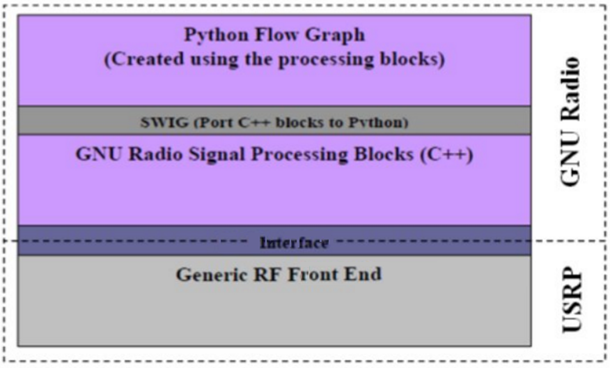
\includegraphics[scale=0.7]{Imagenes/Modelo-SDR.png}
	\label{fig:Modelo-SDR}
		\captionsetup{justification=raggedright,font={scriptsize,bf,it}}
		\caption*{fuente:  El gráfico ha sido adaptado de trabajo: Experimental Study of OFDM Implementation Utilizing GNU Radio and USRP – SDR. Proceedings of the 2009 IEEE 9th Malaysia International Conference on Communications. Kuala Lumpur Malaysia. 15 -17 Diciembre, 2009.
		}
\end{figure}

De este modelo, se puede deducir lo siguiente: \\

\begin{itemize}
	\item [$\bullet$]GNU Radio está compuesto de dos capas que cooperan:	
	\begin{itemize}
		\item [$\bullet$] GNU Radio Signal Processing Blocks (C++). Es una librería en C++ que contiene todos los desarrollos comunes a ser utilizados en programación en el lenguaje C++.
		\item [$\bullet$] Python Flow Graph. Consiste en un desarrollo hecho para facilitar la programación lenguaje en Python o también la basada en un lenguaje gráfico o Flujogramas.
	\end{itemize}
	\item [$\bullet$] Cuando se programa usando Flujogramas, estos producen el código en Python, usando una librería de GNU Radio en Python. Pero esa librería es importada de C++, de modo que indirectamente se usa la librería GNU Radio de C++. La capa señalada com SWIG es la encargada de realizar la importación de C++ de modo que el desarrollador de Python tenga la sensación de que su trabajo es completamente basado en Python.
	\item [$\bullet$] Desde el punto de vista teórico, la componente de software que se desarrolla, se conecta directamente con el hardware, el cual aparece señalado en la figura anterior como USRP, pero que en términos más genéricos, puede llamarse Front End Genérico de RF. Pero en la práctica se requiere algo más: el hardware está alojado en un computador, el cual puede ser tan grande o tan pequeño como sea posible o incluso estar embebido en el hardware, pero este hecho hace que en la práctica se tenga en realidad dos elementos por conectar: el computador y el hardware que para nuestro ejemplo es un USRP. Por esa razón, se requiere introducir un medio de comunicación para estos dos elementos. Ese medio usualmente está representado en los puertos de comunicación que estos dos elementos tengan como: USB, Ethernet u otros.  En la actualidad, los equipos USRP optan por la opción de puerto Gigabit Ethernet, pero otros tipos de hardware como Realtek RTL2832U, optan por puerto USB. En todo caso, cuando hay un medio de comunicación de por medio, surge la necesidad de desarrollar una capa sobre este medio que se encarga de adaptar la información a este medio. En otras palabras, se requiere un software que llamaremos driver, el cual toma la información que entrega el software de la solución SDR, y la traduce para que pueda viajar por el  protocolo de comunicación. Del lado del Front End se requiere también un driver similar para que la comunicación se dé. Para el caso de los USRP ese driver es conocido com UHD (USRP Hardware Driver)
\end{itemize}



\begin{itemize}
	\item [$\bullet$] GNU Radio es realmente una librería de radiocomunicaciones para lenguaje C++, con una versión en el lenguaje Python. El GRC es un ambiente de programación gráfica que aprovecha esa librería y produce código en Python o en c++.
    \item [$\bullet$] Es de uso libre.
    \item [$\bullet$] Las aplicaciones hechas con gnuradio son muy livianas y pueden llevarse a producción sin que dependan de una plataforma determinada.
     \item [$\bullet$] Es ampliamente usada por científicos y académicos.
\end{itemize}

%%%%%%%%%%%%%%%%%%%%%%%%%%%%%%%%%%%%%%%%%%%%%%%%%%%%

\section{Simulación de señales bandabase}

Podría decirse que la Radio Definida por Software representa el uso de la la teoría de señales y sistemas discretos llevada a la práctica. La aplicación práctica implica una relación entre el mundo físico que es por naturaleza continuo y el uso de técnicas de computación que es por naturaleza discreto.\\

Para entenderlo mejor, vamos a volver al sistema de radiodifusión expresado en el modelo de capas de la Figura \ref{fig:ModeloRadiodifusion}. Un sistema de radiodifusión es por su origen analógico tanto por la naturaleza del mensaje como de los equipos usados y la señal emitida. Sin embargo, con los avances tecnológicos, las soluciones que hoy se tienen en el mercado combina tecnología digital y analógica, ya que no tiene lógica alguna usar hoy tecnología analógica para crear un sistema de comunicación por el solo hecho de que ese sistema es analógico. Es por esa razón que cuando hacemos una visita a los estudios de una emisora AM o FM encontramos que todos los equipos nuevos son digitales, aunque AM y FM son modulaciones analógicas.\\
Para entenderlo mejor, en la Figura \ref{fig:ModeloRadiodifusionSDR} se presenta un modelo de capas para un  sistema de radio difusión analógico implementado con tecnología digital, que en realidad es una combinación de tecnologías analógicas y digitales. La combinación se realiza de la siguiente manera:

%\setcounter{figure}{0}
%\vspace{200px}
\begin{figure}[h!]
	\captionsetup{justification = raggedright, singlelinecheck = false}
	\caption{Modelo de capas de un sistema de radio difusión analógico implementado con tecnología digital} 
	\centering
	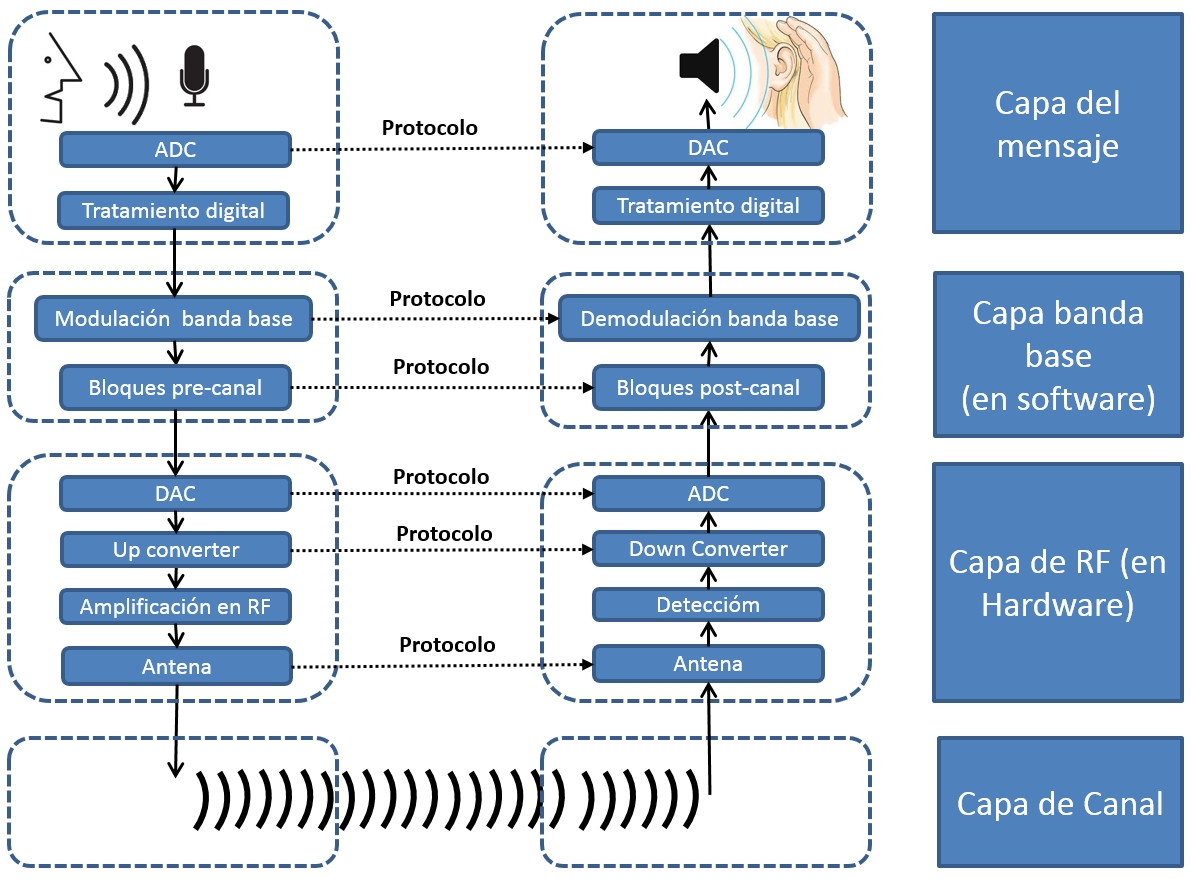
\includegraphics[scale=0.45]{Imagenes/ModeloRadiodifusionSDR}
	\label{fig:ModeloRadiodifusionSDR}
\end{figure}

\begin{itemize}
	\item [$\bullet$] Se conserva la naturaleza analógica del mensaje y de la señal emitida.
    \item [$\bullet$] Tan pronto se tiene la señal del mensaje, se traduce a datos mediante un conversor Análogo Digital (ADC). Este proceso implica el uso de algunos conceptos como el Teorema de Nyquist para realizar un muestreo adecuado a la señal; la cuantificación; la codificación PCM (del inglés Pulse Code Modulation).
    \item [$\bullet$] Lo que sigue es el uso de métodos numéricos que se implementan en un equipo de cómputo tanto para realizar un tratamiento digital del sonido del mensaje pero también, realizar la modulación. 
    \item [$\bullet$] En lugar de usar frecuencias intermedias, la modulación se realiza en banda base, que equivale a obtener una señal que tenga el mismo espectro de la señal modulada tradicionalmente, pero ahora, centrado en la frecuencia cero. 
    \item [$\bullet$] Lo anterior implica nuevos retos teóricos y técnicos, pues la señal modulada en banda base resulta ser compleja y se conoce como la Envolvente Compleja
    \item [$\bullet$] El reto teórico consiste en la necesidad de saber modular y demodular señales usando el concepto de Envolvente Compleja
    \item [$\bullet$] El reto técnico aparece con la capa que hemos llamado Capa RF, donde predominan tareas con equipo analógico analógicas. Antes de entregar la señal a esta capa es necesario preparar la señal para su paso a un medio analógico, eso es lo que hemos llamado Bloques Pre-canal. Luego, la señal pasa al dominio continuo usando un Conversos Digial Análogo (DAC).
    \item [$\bullet$] El Up converter es un circuito que permite mover el espectro de la señal recibida para que quede centrado en la frecuencia RF.
    \item [$\bullet$] La antena simplemente traduce la señal eléctrica en señal obtenida en señal electromagnética
    \item [$\bullet$] Es claro que en la parte receptora se tienen componentes que hacen pareja con los mencionados anteriormente, para recibir la señal, desplazar el espectro de esa señal a la frecuencia cero, usando un Down Converter y así sucesivamente.\\

Este modelo deja precisamente claro la tendencia natural para la implementación de los futuros sistemas de comunicaciones basados en Software Defined Radio (SDR). Básicamente, un sistema de SDR tiene las siguientes características:

    \item [$\bullet$] Tienen una componente de software y una de hardware
    \item [$\bullet$] En la componente de hardware se realiza unas tareas que son comunes para cualquier sistema de comunicaciones: mover la señal en el dominio de las frecuencias para centrarla en la frecuencia RF, amplificarla de acuerdo a las necesidades, transmitirla en forma de ondas de radio. En fin, la componente de hardware corresponde a la Capa RF en la Figura \ref{fig:ModeloRadiodifusionSDR}. Las prácticas propuestas en este libro se apoyan mayormente en un hardware SDR de National instruments conocido como USRP.
    \item [$\bullet$] La componente de software se aloja en un computador y es allí donde se implementan soluciones para sistemas específicos de comunicaciones. A diferencia de lo que ocurre en los sistemas analóticos, los métodos que aquí se implementan son muy cercanos a los teóricos, por ejemplo, una modulación FM puede estar dada por una o varias fórmulas o por uno o más algoritmos. 
    \item [$\bullet$] En la componente de software la programación se realiza para señales banda base, para lo cual existen diversas herramientas de programación. La que usaremos en el presente libro se conoce como gnuradio. Se trata principlamente de una librería que reune las experiencias en el tema de una gran comunidad de desarrolladores
    \item [$\bullet$] Al lado de gnuradio, también se cuenta con una herramienta conocida como GRC, que permite realizar la programación gráfica, usando bloques, de manera similar a lo que se puede lograr usando Simulink de Matlab. De hecho, Simulink de Matlab también puede ser usada para implementar soluciones SDR.
\end{itemize}

\subsection{La Conversión Análogo Digital}
Como se vió anteriormente, en la parte transmisora se requiere usar un dispositivo ADC y en la receptora un dispositivo DAC. Puede decirse que estos elementos sirven de compuerta entre el mundo continuo y el digital. Conocer muy las capacidades y las limitaciones que tienen estos dispositivos es clave para poder lograr un montaje funcional. A continuación se revisan los principales procesos y características de un ADC:

\subsubsection{El muestreo. La frecuencia de muestreo y el ancho de banda}

El ADC puede ser visto como un medidor de la tensión de una señal, que mide en tiempos discretos separados entre sí en un tiempo $T_s$. Por lo tanto, las mediciones se presentan a la frecuencia de muestreo $F_s=\frac{1}{T_s}$.\\

Los siguientes son los aspectos que merecen mayor atención: \\
\begin{itemize}
	\item [$\bullet$] De acuerdo al Teorema de Nyquist, la señal muestreada puede llegar a tener una frecuencia máxima igual a $F_{max}=\frac{F_s}{2}$ se tiene el principal parámetro. Eso significa que un un ADC está limitado en ancho de banda.
    \item [$\bullet$] El costo en dinero que puede tener un ADC se eleva exponencialmente con la frecuencia de muestreo que soporte.
    \item [$\bullet$]  El muestreo es un proceso reversible, al menos desde el punto de vista teórico siempre y cuando la señal haya sido muestreada respetando el Teorema de Nyquist. \\
    
La puesta en práctica del Teorema de Nyquist es lo que produjo en los año 60 la revolución PCM, que es cuando la telefonía, siendo la red más grande del mundo adoptó la tecnología PCM en toda su dimensión. La idea consistía en tomar la señal de voz de un teléfono, limitar su ancho de banda hasta 4 kHz, muestrearla a una frecuencia de muestreo de 8 kHz, con lo cual el periodo de muestreo o distancia de muestra y muestra sería de $125 \mu seg$ . Esa distancia de tiempo entre muestra y muestra se aprovechó para enviar allí muchas más señales de voz también muestreadas. Se elevó entonces la capacidad de las redes, pues ya no era necesario tener un par de hilos de cobre entre dos puntos para conducir cada llamada teléfonica, pues muchas llamadas telefónicas podían ahora viajar sobre un mismo par de hilos de cobre.\\

Usualmente los estudiantes no se convencen del mensaje que envía el Teorema de Nyquist y que puede enunciarse así: si tu muestreas una señal usando una frecuencia de muestre que sea igual o superior a dos veces la frecuencia máxima que esa señal pueda llegar a tener, siempre podrás recuperar, sin pérdida alguna, la forma continua de esa señal a partir de la versión discreta. Ósea que el proceso de muestreo para de dejar de transmitir la señal todo el tiempo y hacerlo solo por instantes, no implica que la señal continua haya dejado de existir. \\

    
\end{itemize}
\subsubsection{La cuantificación. El Diapasón de cuantifiación}
En un ADC La cuantificación es inseparable del proceso de muestreo. Surge debido a que un ADC nunca puede llegar a entregar una señal muestreada como la que teóricamente esperamos. Esto es debido a las siguientes posibles razones:
\begin{itemize}
	\item [$\bullet$] La salida del ADC es un número acotado en bits. Algunos pueden permitir una configuración, por ejemplo para usar 32 bits/muestra o 64 bits/muestra. Los usados en telefonía fija deben cumplir una recomendación de la UIT-T que establece que son 8 bits/muestra 
    \item [$\bullet$]Por lo anterior, el proceso de cuantificación equivale a una una especie de muestreo en amplitud. Pero la cuantificación no es un proceso reversible como sí lo es el muestreo cuando se cumple el Teorema de Nyquist. \\
    
En la Figura \ref{fig:3_bit_cuantizacion} se presenta una comparación entre una señal continua y su versión cuantificada a la razón de 3 bits/muestra.

\begin{figure}[h!]
	\captionsetup{justification = raggedright, singlelinecheck = false}
	\caption{Comparación entre una señal continua y una cuantificada a la razón de 3 bits/muestra} 
	\centering
	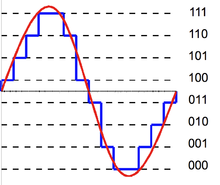
\includegraphics[scale=1]{Imagenes/3-bit_cuantizacion}
	\label{fig:3_bit_cuantizacion}
\end{figure}
    \item [$\bullet$]Por lo anterior, un ADC tiene unos límites inferior y superior para la amplitud de la señal que puede entregar
    \item [$\bullet$]Pero algo no menos relevante es que un ADC también tiene unos límites inferior y superior para la señal que recibe. La diferencia entre esos dos limites es lo que se conoce como Diapasón de cuantificación.
    \item [$\bullet$]Los siguientes son los problemas más comunes con el uso de ADC:
    \begin{itemize}
		\item [$\bullet$] La señal que entra al ADC puede ser tan débil que la cuantificación la deforma completamente porque queda expresadas con muy pocos niveles de amplitud.
        \item [$\bullet$] La señal que entra al ADC puede ser tan fuerte que se sale del diapason que soporta, de modo que las amplitudes que se salen del diapasón desaparecen deformando la señal.
        \item [$\bullet$] La señal entrante puede tener un ancho de banda que supera el soportado por el ADC, lo cual hace que la señal resulte irrecuperable.
    	\item [$\bullet$]\textcolor{Red}{El resultado de la ...}
	\end{itemize}
      
\end{itemize}

\subsection{El paso a un código de línea. PCM}

\subsection{La Conversión Digital Análoga}
La Conversión Digital Análoga es el proceso inverso de la Conversión Análoga Digital. En este sentido, el DAC tiene parámetros similares al ADC.

\subsection{Filtros digitales}
\textcolor{Red}{[falta]. }\\

La idea es explicar lo que significan los filtros digitales. Básicamente como un sistema LIT con una respuesta al impulso

\subsection{interpoladores}
\textcolor{Red}{[falta]}
\subsection{Decimadores}
\textcolor{Red}{[falta]}

\subsection{Transformada Rápida de Fourier (FFT)}
Se trata de un algoritmo que permite calcular, con un óptimo recurso computacional, la siguiente fórmula.

\begin{equation} \label{capdos}
	 C_{k} =  \sum_{n=0}^{N-1}x_{N} [n]e^{-j2 \pi kn/N}
\end{equation}

\subsubsection{Aspectos relevantes de aplicación práctica:}
El uso de la FFT en la práctica pasa por las siguientes consideraciones:
\begin{itemize}
	\item  [$\bullet$] La FFT puede servir para obtener la RSF de una señal de la siguiente manera:
	\begin{itemize}
		\item [$\bullet$]  Si x[n] proviene de una señal continua, el muestreo debe haber sido realizado respetando el Teorema de Nyquist.
		\item [$\bullet$]  La señal debe ser periódica en N.
		\item [$\bullet$]  La FFT se aplica una única vez, para N, con lo cual se produce un espectro estático.
		\item [$\bullet$]  El espectro obtenido debe ser dividido en N.
	\end{itemize}
	\item [$\bullet$] La FFT puede servir para obtener una aproximación de la TF de una señal de la siguiente manera:
	\begin{itemize}
	\item [$\bullet$]  Si x[n] proviene de una señal continua, el muestreo debe haber sido realizado respetando el Teorema de Nyquist. 
	\item [$\bullet$]  Ente más grande sea N, la aproximación será mejor. Es claro que si N es exageradamente grande, resulta engorroso tener que esperar mucho tiempo para obtener el resultado, además la resolución que se obtiene puede ser exagerada para nuestras necesidades reales.
	\end{itemize}

	\item [$\bullet$]  La FFT puede servir para obtener un espectro dinámico o instantáneo de una señal de la siguiente manera
		\begin{itemize}
	\item [$\bullet$]  Con las muestras de x[n] se van creando paquetes de N muestras. N no debe ser tan grande, se recomienda que sea igual al número de puntos que su ojo podría distinguir en la pantalla de su computador, por ejemplo N=1024 o N=512
	\item [$\bullet$]  Se aplica la FFT a un paquete de N muestras para obtener N muestras espectrales. Luego se obtiene la magnitud al cuadrado y se convierte a dB 
	\item [$\bullet$]  Se repite lo anterior para cada uno de los subsiguientes paquetes, con lo cual en la pantalla veremos un espectro que va variando en el tiempo.
		\end{itemize}
	\item [$\bullet$]  La FFT puede servir para obtener la PSD si se aplica de la siguiente manera:
		\begin{itemize}
		\item [$\bullet$]  Se hace lo mismo que el caso anterior, pero cada paquete de N muestras espectrales se va promediando con los anteriormente recibidos.
		\end{itemize}
\end{itemize}
\subsection{La IFFT}
Representa el mecanismo inverso a la FFT. Por lo tanto se apoya en la ejecución de la siguiente fórmula:\\

\begin{equation} \label{capdos_uno}
	 x_{N}[n] =  \sum_{k=0}^{N-1}C_{k}e^{j2 \pi kn/N}
\end{equation}
%\vspace{30px}

\subsection{Simulación de un analizador de espectros}

Analizaremos dos bloque que tiene GNU Radio y que usan la FFT: El bloque FFT y el bloque QT GUI Frequency Sink. En la figura \ref{fig:la-FFT} 

\begin{figure}[h!]
	\captionsetup{justification = raggedright, singlelinecheck = false}
	\caption{Flujograma La-FFT.grc. Comparación del bloque FFT con QT GUI Frequency Sink para observar la PSD de una señal binaria bipolar aleatoria.} 
	\centering
	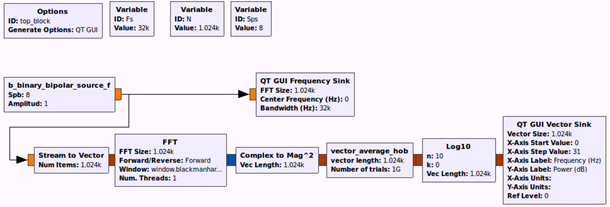
\includegraphics[scale=1]{Imagenes/La-FFT.png}
	\label{fig:la-FFT}
	%		\captionsetup{justification=raggedright,font={scriptsize,bf,it}}
	%		\caption*{fuente: http://superkuh.com/rtlsdr.html}
\end{figure}

La siguiente figura presenta el resultado del bloque QT GUI Frequency Sink

%\vspace{100px}
\begin{figure}[h!]
	\captionsetup{justification = raggedright, singlelinecheck = false}
	\caption{PSD obtenida usando QT Frequency Sink.} 
	\centering
	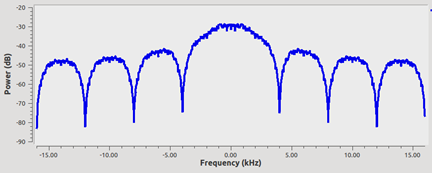
\includegraphics[scale=1]{Imagenes/PSD-QT.png}
	\label{fig:la-PSD-QT}
	%		\captionsetup{justification=raggedright,font={scriptsize,bf,it}}
	%		\caption*{fuente: http://superkuh.com/rtlsdr.html}
\end{figure}

La figura \ref{fig:la-PSD-FFT} presenta el resultado del bloque FFT.

\vspace{200px}
\begin{figure}[h!]
	\captionsetup{justification = raggedright, singlelinecheck = false}
	\caption{PSD obtenida usando el bloque FFT combinado con otros bloque} 
	\centering
	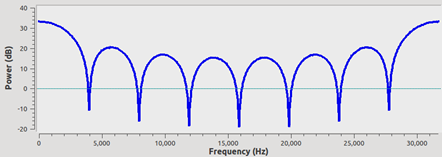
\includegraphics[scale=1]{Imagenes/PSD-FFT.png}
	\label{fig:la-PSD-FFT}
	%		\captionsetup{justification=raggedright,font={scriptsize,bf,it}}
	%		\caption*{fuente: http://superkuh.com/rtlsdr.html}
\end{figure}

Conclusiones de las observaciones y recomendaciones para usar estos bloques:

\begin{itemize}
	\item [$\bullet$]  Obtener la PSD usando el bloque FFT requiere preparar el vector, pasar el resultado de la FFT a magnitud al cuadrado, realizar un promediado con los vectores previos, convertir a dB y graficar. 
	\item [$\bullet$]  Aunque parezca diferente, la imágen obtenida con el bloque FFT es equivalente a la del bloque QT GUI Frequency Sink, ya que la teoría de Fourier dice que la Transformada de Fourier Discreta (DFT) es periódica en $F_{r}= 2\pi Rad/seg$ y eso significa que es periódico en la frecuencia de muestreo $F_{s}$ (Hz)de la señal vista en el tiempo. Por eso, si el bloque FFT pudiese ser configurado para que muestre el espectro entre $\dfrac{-F_{s}}{2}$ y $\dfrac{F_{s}}{2}$ tendríamos imágenes similares. La imágen obtenida con el bloque FFT es más continua debido a que el bloque vector-average-hob, usado como complemento al bloque FFT realiza un promediado más prolongado.
	\item  [$\bullet$] La frecuencia máxima que puede mostrar un Analizador de Espectros es igual a la frecuencia de muestreo sobre 2. También puede observarse que el ancho de banda B, que abarca tanto frecuencias negativas como positivas, es igual a la frecuencia de muestreo.
	\item [$\bullet$]  N es el tamaño del vector y es igual al orden de la FFT, también es igual al número de puntos que son graficados en la ventana. De deduce que la resolución espectral es 	$ f_{Resol} = \dfrac{frecuencia de muestreo}{N}$
	\item [$\bullet$]  Finalmente, es importante tener en cuenta que la PSD se calcula usualmente a señales que son parte del mundo continuo, por ejemplo la señal que se emite desde un transmisor, la que se recibe en un receptor, la que produce un micrófono o la que usa una bocina. Desde este punto de vista, no es usual buscar la PSD de señales que pueden encontrarse en bloques intermedios como por ejemplo un codificador o un modulador digital bandabase.	
\end{itemize}

%%%%%%%%%%%%%%%%%%%%%%%%%%%%%%%%%%%%%%%%%%%%%%%%%

\section{Simulación de señales paso bandas}



\subsection{La Modulación AM}

\textcolor{red}{[Falta: Oscar Reyes]} %\OR a nivel de flujograma??

\subsection{La Modulación FM}

\textcolor{red}{[Falta: Oscar Reyes]}


\subsection{El heterodinado}
\textcolor{red}{[Falta: Oscar Reyes]}

\subsection{Conversión RF}

La Conversión RF es un término que se está introduciendo en este libro, por lo tanto, no lo encontrará en ninguna otra fuente anterior a esta. Se refiere al proceso de pasar una señal real de su correspondiente Envolvente Compleja (EC) y viceversa. La razón para introducir este concepto es meramente pedagógica y consiste en lo siguiente: cuando un ingeniero trabaja con GNU Radio, estará operando casi siempre con la EC, mientras la señal que viaja entre las antenas es pasobandas. La forma en que se define a continuación la Conversión RF ayuda a que ese ingeniero pueda realizar una traducción muy sencilla entre lo que ve en GNU Radio y lo que viaja entre las antenas sin importar qué tipo de modulación se esté usando. Así, si en la señal pasobandas se observa una variación de la amplitud de la onda senoidal, entonces en GNU Radio se observará una variación similar en la magnitud de la envolvente compleja. Algo similar puede decirse de la frecuencia de la fase. Es importante tener en cuenta que una señal pasobandas, recibida por una antena, para ser transformada en una onda electromagnética es siempre senoidal, de modo que la envolvente compleja es siempre una función de euler compleja.\\

\subsection{Conversión RF Directa en el dominio del tiempo}

\begin{equation} \label{equ_rfc}
A(t)\cos{ 2 \pi[f_{c}+B(t)]t+Q(t)} \ 
%	\overrightarrow{Conversión \ RF}
\overset{Conversion \ RF}{\rightarrow}
A(t) e^{j[2\pi B(t)t+Q(t)]}
\end{equation}

La señal que se obtiene en esta conversión se conoce como Envolvente Compleja

\subsection{Conversión RF Inversa  en el dominio del tiempo}

\begin{equation} \label{equ_frc_inv}
A(t)e^{j[2\pi B(t)t+Q(t)]} \
\overset{Conversion \ Inversa \ RF}{\rightarrow} \ A(t)\cos{ 2 \pi[f_{c}+B(t)]t+Q(t) } 
\end{equation}

\subsection{La Conversión RF en el dominio de las frecuencias}

\begin{figure}[h]
	\captionsetup{justification = raggedright, singlelinecheck = false}
	\caption{La Conversión RF en el dominio de las frecuencias. \textcolor{red}{corregir: en la gráfica con se notan las letras, están muy diminutas}} 
	\centering
	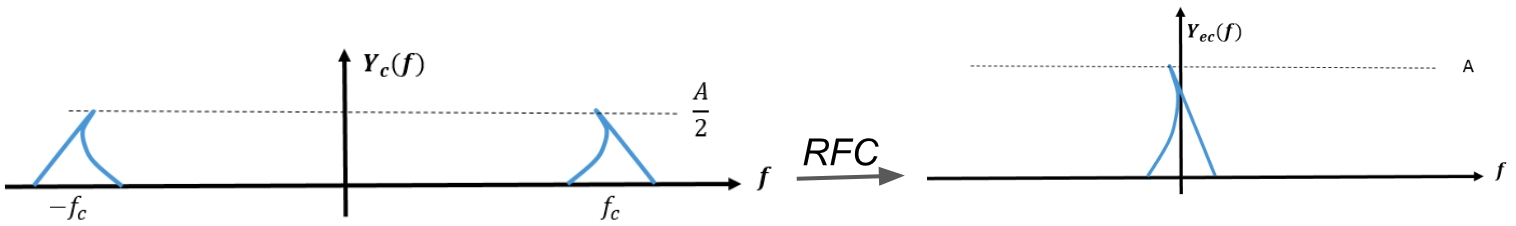
\includegraphics[scale=0.25]{Imagenes/rfconversion.jpg}
	\label{fig:RTC}
	%	\captionsetup{justification=raggedright,font={scriptsize,bf,it}}
	%	\caption*{fuente: llllll}
\end{figure}

\subsection{El Up Converter}
Puede verse como una solución práctica de la Conversión RF inversa y se presenta en la siguiente figura \\

\vspace{200px}
\begin{figure}[h!]
	\captionsetup{justification = raggedright, singlelinecheck = false}
	\caption{Up converter.\textcolor{red}{corregir: las fórmulas de la figura no se ha puesto como fórmulas}} 
	\centering
	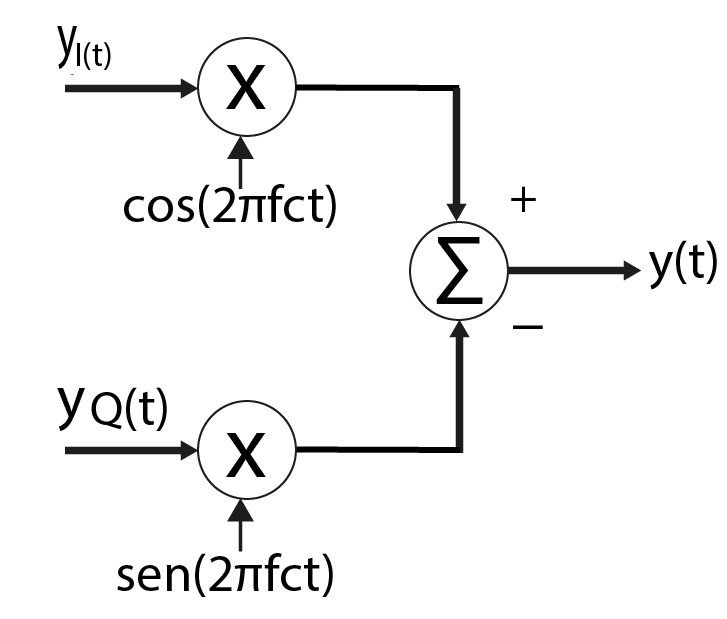
\includegraphics[scale=0.3]{Imagenes/Up.png}
	\label{fig:Up}
%	\captionsetup{justification=raggedright,font={scriptsize,bf,it}}
%	\caption*{fuente: llllll}
\end{figure}

\textbf{Ejercicio:} Hallar la expresión de la Envolvente Compleja de una señal FM paso bandas. Es bien sabido que la expresiòn matemàtica de una señal pasobandas FM es:\\

	\begin{equation} \label{capdos_cinco}
		s(t)= A_{c}\cos(2\pi(f_{c}+K_{f}m(t))t )  %\OR la expresión no es correcta
	\end{equation}

Donde, $A_{c}$ es la amplitud de la portadora, $f_{c}$ es la frecuencia de la portadora, $K_{f}$ es el coeficiente de modulación, $m(t)$ es el mensaje y $t$ es la variable de tiempo.\\

\textbf{Solución}: La siguiente figura presenta una forma hipotética de la TF de $s(t)$.\\

\begin{figure}[h!]
	\captionsetup{justification = raggedright, singlelinecheck = false}
	\caption{Espectro de señal paso bandas.} 
	\centering
	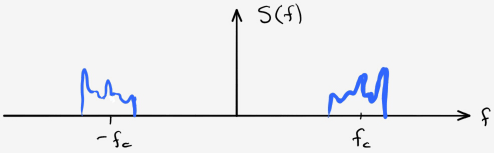
\includegraphics[scale=1]{Imagenes/Espectro-pasobanda.png}
	\label{fig:Espectro-pasobanda}
	%	\captionsetup{justification=raggedright,font={scriptsize,bf,it}}
	%	\caption*{fuente: llllll}
\end{figure}

Obtenemos la expresión para la señal $s(t)$ cuya TF es la misma $S(f)$ pero sin  la componente en frecuencias negativas, como  siguiente figura \\

\vspace{200px}
\begin{figure}[h!]
	\captionsetup{justification = raggedright, singlelinecheck = false}
	\caption{Espectro de la Pre envolvente compleja.} 
	\centering
	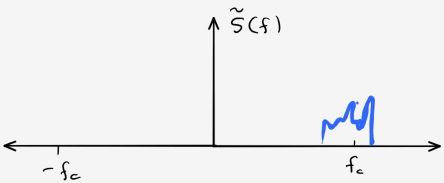
\includegraphics[scale=1]{Imagenes/Espectro-pre.png}
	\label{fig:Espectro-pre}
	%	\captionsetup{justification=raggedright,font={scriptsize,bf,it}}
	%	\caption*{fuente: llllll}
\end{figure}

$s(t)= \frac{1}{2}A_{c}e^{j(2\pi(f_{c}+K_{f}m(t)t))}.$ Esta expresión debe multiplicarse por 2 para conservar la energía, con lo cual se obtiene la pre-envolvente compleja. Hacemos $f_{c}=0$ y obtenemos la Envolvente Compleja.\\ 

\begin{equation} \label{capdos_seis}
	Sec(t)= A_{c}e^{j(2\pi(K_{f}m(t))t)} = A_{c}\cos(2\pi 0K_{f}m(t)t) + jA_{c}\sin(2\pi 0K_{f}m(t)t) 
\end{equation}

Esta es a su vez la fórmula de la FM bandabase. En principio, a cualquier señal pasobandas le corresponde una versión bandabase , que es su envolvente compleja. Podemos ver que la envolvente compleja de una señal FM es un vector rotante. En el sitio web del libro se brindan más detalles en forma de vídeos demostrativos sobre Envolvente Compleja y Up converter.\\

\begin{center}
\url{https://sites.google.com/saber.uis.edu.co/comdig/m/ec} 
\end{center}

\subsection{El Down Converter}

Para obtener la Envolvente Compleja de una señal paso bandas, se usa un dispositivo que llamaremos “Down converter” y que se presenta en la siguiente gráfica: \\

%\vspace{100px}
\begin{figure}[h!]
	\captionsetup{justification = raggedright, singlelinecheck = false}
	\caption{Tomado del Libro de Haykin, cap 1.11.} 
	\centering
	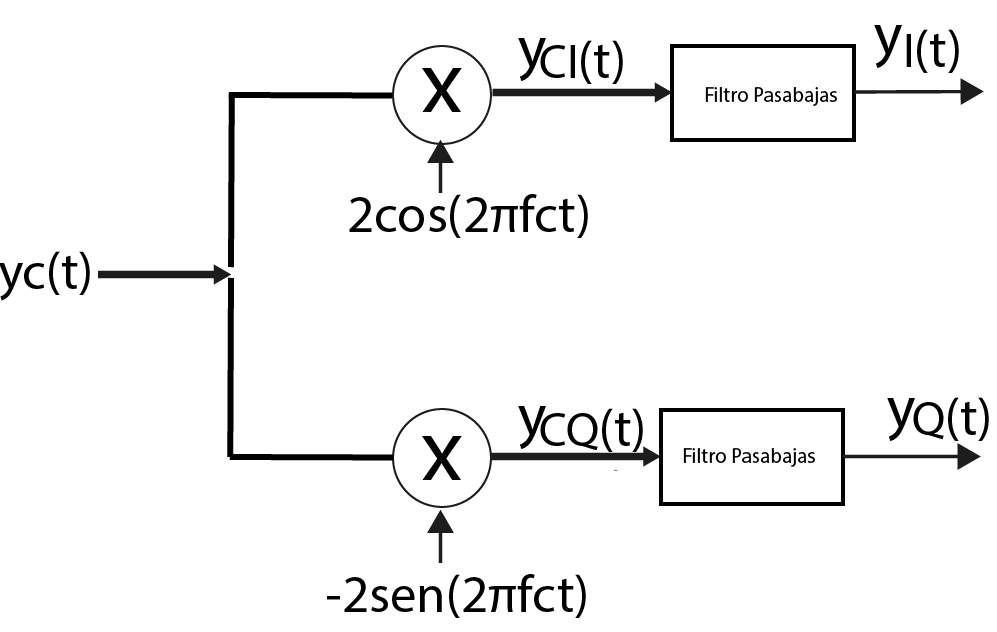
\includegraphics[scale=0.3]{Imagenes/libro-haykin.png}
	\label{fig:libro-haykin}
%	\captionsetup{justification=raggedright,font={scriptsize,bf,it}}
%	\caption*{fuente: http://youtu.be/h-rseLrniCk}
\end{figure}

La envolvente compleja es la señal $y_{c}(t) =  y_{I}(t) + j y_{Q}(t)$,  $y_{I}(t)$ es conocida como la componente en fase,  $y_{Q}(t)$ como la componente en cuadratura de la Envolvente Compleja.

\subsubsection{Demostración del Down Converter}

La Transformada de Fourier es una herramienta útil para diseñar y demostrar la validez de este tipo de soluciones.\\

\begin{equation} \label{capdos_siete}	
y(f)= \frac{1}{2}[y_{ec}(f-f_{c})+y_{ec}(-f-f_{c})]
\end{equation}

\begin{equation} \label{capdos_ocho}
y_{CI}(t) = y_{c}(t)2\cos (2\pi f_{c}t) \Longrightarrow y_{CI}(t) = y_{c}(f-f_{c})+y_{c}(f+f_{c}) 
\end{equation}

\begin{equation} \label{capdos_nueve}
y_{CI}(f) = \frac{1}{2}  [y_{ec}(f-2f_{c}) + y_{ec}(-f) + y_{ec}(f)+y_{ec}(-f-2f_{c})]
\end{equation}

\begin{equation} \label{capdos_diez}
y_{I}(f) = \frac{1}{2}[y_{ec}(-f) + y_{ec}(f)]
\end{equation}

\begin{equation} \label{capdos_once}
y_{CQ}(t) = -2y_{c}(t)\sin (2\pi f_{c}t)  \Longrightarrow TF y_{CQ}(f)= \frac{-1}{2j} [y_{c}(f-f_{c})-y_{c}(f+f_{c})]
\end{equation}

\begin{equation} \label{capdos_doce}
y_{CQ}(f) = \frac{-1}{2j} [y_{ec}(f-2f_{c}) + y_{ec}(-f) - y_{ec}(f)- y_{ec}(-f-2f_{c})]
\end{equation}

\begin{equation} \label{capdos_trece}
y_{Q}(f) = \frac{1}{2j} [y_{ec}(f)- y_{ec}(-f)]
\end{equation}

De modo que el sistema de la figura \ref{fig:libro-haykin} permite obtener la componente en fase y cuadratura de la Envolvente Compleja $y_{ec}(t) \Longrightarrow  y_{ec}(f)$

\subsubsection{Demostración gráfica del Down Converter}

Aplicaremos el Down Converter de la figura \ref{fig:Up} a la señal que tiene la TF de la figura \ref{fig:Espectro-bandapaso}. Deberemos obtener la TF de la Envolvente Compleja que es la que aparece en la figura \ref{fig:Espectro}.

%\vspace{100px}
\begin{figure}[h!]
	\captionsetup{justification = raggedright, singlelinecheck = false}
	\caption{Resultado del uso del Down Converter} 
	\centering
	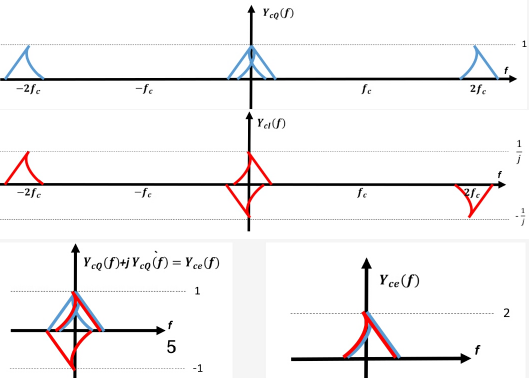
\includegraphics[scale=0.9]{Imagenes/resultado.png}
	\label{fig:resultado-down}
%	\captionsetup{justification=raggedright,font={scriptsize,bf,it}}
%	\caption*{fuente: http://youtu.be/h-rseLrniCk}
\end{figure}


\subsection{La Envolvente compleja. Sus características}
\subsubsection{El problema a resolver}

A continuación se enuncia un problema que justifica el uso de este concepto.\\

Deseamos implementar un analizador de espectros  en un computador portátil mediante una aplicación basada en la FFT. Observar el espectro de la voz usando la FFT no representa un gran problema. Necesitamos conectar un micrófono al computador, el cual tiene un ancho de banda que finalmente establece una frecuencia máxima para la voz. Cumpliendo el Teorema de Nyquist, la señal de voz deberá ser muestreada a la frecuencia de muestreo \\ 

\begin{equation} \label{capdos_catorce}
f_{s} \geq 2f_{max} = 30KHz
\end{equation}

EL problema se complica cuando se desea analizar la señal que proviene de la radio base de un operador móvil. Será necesario conectar un receptor que convierte la señal electromagnética en una señal eléctrica y la amplifica de manera suficiente. \\ 

%\vspace{200px}
\begin{figure}[h!]
	\captionsetup{justification = raggedright,singlelinecheck = false}	
    \caption{Analizador de espectros basado en computador.} 
    \label{fig:Analizador}
    \centering
    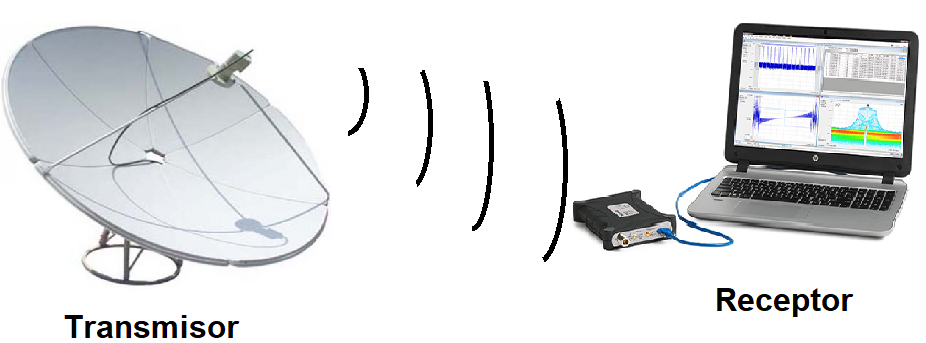
\includegraphics[trim = 0mm 0mm 0mm 0mm, clip,width=1\textwidth]{Imagenes/Analizador}
	\par
		\captionsetup{justification=raggedright,font={scriptsize,bf,it}}
		\caption*{fuente: Autor}
\end{figure}

Pero ahora tenemos una frecuencia máxima muchísimo mayor, por ejemplo 1900000000 Hz. De modo que el muestreo resulta ahora extremadamente costoso y la FFT debe desarrollar tantas operaciones que el espectro no podrá ser visto en tiempo real. \\ 

\subsubsection{La solución. La Envolvente compleja}

{\setlength{\parindent}{1pt}La solución lógica consiste en incluir dentro  del receptor un dispositivo que permita desplazar el espectro de la señal de interés para centrarlo en una frecuencia mucho más baja a la que estaba centrado originalmente. El caso más extremo se tiene cuando el receptor logra centrar el espectro en $f_{c}$= 0 Hz.}  \\ 

{\setlength{\parindent}{1pt} En la siguiente gráfica se representa un ejemplo de la Transformada de Fourier de la señal de interés }

\vspace{200px}
\begin{figure}[h!]
	\captionsetup{justification = raggedright, singlelinecheck = false}
	\caption{Espectro de la señal pasobandas de interés.} 
  	\label{fig:Espectro-bandapaso}
	\centering
	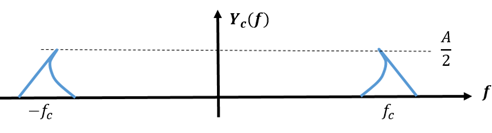
\includegraphics[trim = 0mm 0mm 0mm 0mm, clip,width=1\textwidth]{Imagenes/Espectro-bandapaso.png}
	%	\captionsetup{justification=raggedright,font={scriptsize,bf,it}}
	%	\caption*{fuente: llllll}
\end{figure}


{\setlength{\parindent}{1pt}En la figura \ref{fig:Espectro-bandapaso}, el espectro es simétrico alrededor de la frecuencia $f = 0 Hz$, por lo tanto pertenece a una señal real. Sin embargo, alrededor de la frecuencia fc no es simétrico lo cual es usual  en las comunicaciones. 
En la figura \ref{fig:Espectro} se muestra el resultado al que queremos llegar, donde el espectro aparece centrado en $f_{c}=0 Hz$. Tiene doble amplitud que el de la  figura \ref{fig:Espectro-bandapaso}, con el fin de que conserve la misma energía.} \\ 

\begin{figure}[h!]
	\captionsetup{justification = raggedright, singlelinecheck = false}
	\caption{Espectro de la Envolvente Compleja.} 
	\centering
	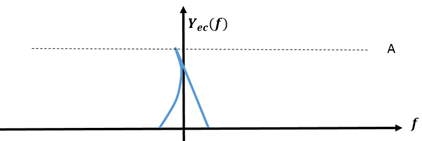
\includegraphics[scale=1.2]{Imagenes/Espectro-envolvente.png}
	\label{fig:Espectro}
	%	\captionsetup{justification=raggedright,font={scriptsize,bf,it}}
	%	\caption*{fuente: llllll}
\end{figure}

{\setlength{\parindent}{1pt}Pero ahora el espectro no es simétrico, luego pertenece a una señal compleja que llamaremos Envolvente Compleja.Puede decirse que la Envolvente Compleja es la señal que resulta en el dominio del tiempo al desplazar el espectro de una señal paso bandas de interés que está centrado en una frecuencia $f_{c}$ $>$ 0 para que quede centrado en la frecuencia  $f_{c}$= 0 Hz, sin que se afecte la forma del espectro y por lo tanto sin que se afecte la información que está contenido en él.}\\

\subsection{El uso de la envolvente compleja en la simulación de Sistemas de comunicaciones}

El problema que en este caso justifica el uso de la Envolvente Compleja es el siguiente: supongamos que un operador móvil tiene instalada una red de datos inalámbrica por toda la ciudad y ahora desea cambiar el sistema de comunicación usado a otro. Por ejemplo, pasar de 2G a 3G.  Bien podría reutilizar la red de radio ya instalada. Entonces solo adquirir comparar la sección de equipos que procesa la Envolvente Compleja, que a menudo también se conoce como la señal banda base o componente en fase y en cuadratura ó señal I y señal Q. La sección de radio, en la parte transmisora, se encarga de obtener la señal paso bandas a partir de la envolvente compleja. En la parte receptora, esta sección se encarga de obtener la señal banda base a partir de la paso bandas. En otras palabras, la sección de radio incorpora un up-converter en la parte transmisora y un down-converter en la parte receptora. \\

\vspace{100px}
%\setcounter{figure}{11}
\begin{figure}[h!]
	\captionsetup{justification = raggedright, singlelinecheck = false}
	\caption{Esquema de Modulación pasobandas usando SDR} 
	\centering
	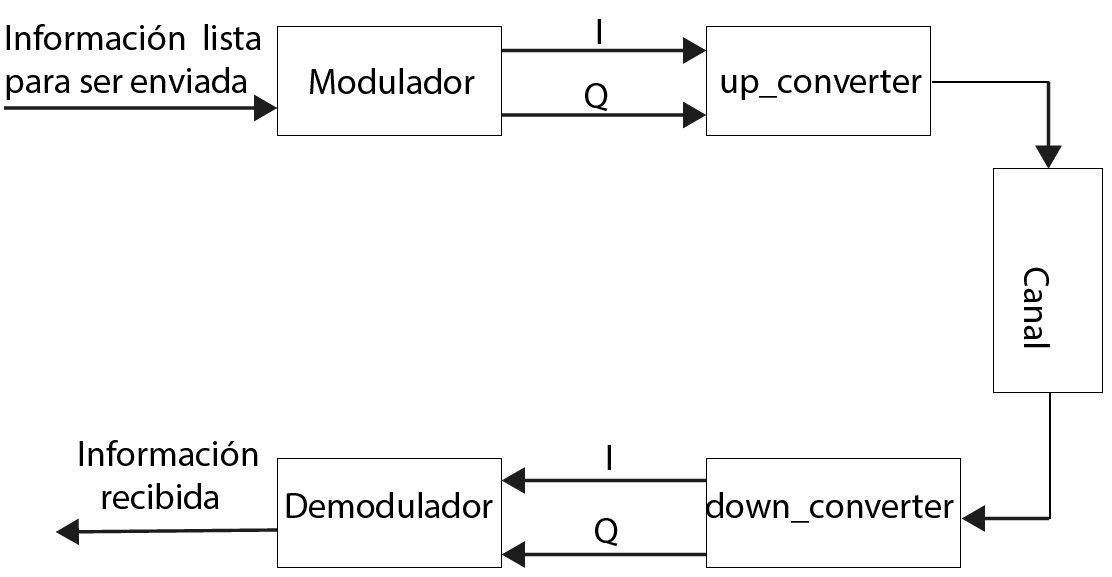
\includegraphics[scale=0.3]{Imagenes/Envol-GNU.png}
	\label{fig:Envol-GNU}
	%	\captionsetup{justification=raggedright,font={scriptsize,bf,it}}
	%	\caption*{fuente: http://youtu.be/h-rseLrniCk}
\end{figure}

En GNU Radio, la EC sólo puede generarse, observarse y recibirse en forma de una señal discreta. Esto obliga a tener ciertos cuidados principalmente relacionados con la frecuencia de muestreo. Los siguientes son puntos a tener en cuenta:\\

\begin{itemize}
	\item [$\bullet$] El modelo matemático de la EC en forma discreta es: $S_{ec}(t) = A[n]e^{j[2\pi B(n)n/B +Q(n) ]}$ y es de esta forma que puede ser implementado el modulador. El parámetro $N$ está relacionado con la frecuencia de muestreo samp-rate y este último con el tiempo continuo, así: \\
	$samp-rate=T/N$, donde $T$ es el periodo de la frecuencia máxima que puede tener la señal y $N$ es el número de muestras en ese periodo.
	\item [$\bullet$] Algunos bloques pueden producir la fórmula anterior, sin que el programador tenga que ver con esa expresión, por ejemplo el bloque Signal Source, pide parámetros continuos como la amplitud, la frecuencia y por supuesto la frecuencia de muestreo.
	\item [$\bullet$] Un modulador usualmente usa solo uno o dos de los anteriores parámetros de modo que la ecuación se puede simplificar en varias formas como las siguientes:	
	\begin{itemize}
		\item [$\bullet$] Cuando solo varía la magnitud: $S_{ec}(t)= A[n]$	
		\item [$\bullet$] Cuando solo varía la fase: $S_{ec}(t)= e^{jQ(n)}$
		\item [$\bullet$] Cuando varía fase y amplitud: $S_{ec}(t) = A[n]e^{jQ(n)}$
		\item [$\bullet$] Cuando solo varía la frecuencia: $S_{ec}(t) = e^{j2\pi B(n)n/N }$
	\end{itemize}
   
	\item [$\bullet$] Luego del modulador, al interior del USRP se cuenta con un elemento que llamamos “Complex to Real” que convierte la EC en dos señales, la señal I y la señal Q, también conocidas como señal en fase y señal en cuadratura.
	\item [$\bullet$] Esas dos señales entran luego a un DAC donde se convierten en señales eléctricas continuas. Es aquí donde la frecuencia de muestreo de la señal que se entrega al DAC juega un gran papel para llegar a producir de manera apropiada esas señales continuas. Básicamente debe cumplirse el Teorema de Nyquist.	
	\item [$\bullet$]Puede decirse que a la salida del DAC se tiene la EC en forma continua, pero en forma de dos señales reales, la señal I y la señal Q.
	\item [$\bullet$] Finalmente, el Up Converter aplica en el plano continuo lo que arrima hemos llamado Conversión RF.
\end{itemize}

En la parte receptora ocurre algo similar en sentido contrario . \\


\subsection{Simulación de señales y sistemas de comunicación en versión bandabase}

Es similar a lo explicado anteriormente, pero el canal también se simula en versión banda base de modo que no se hace necesario incluir un Up Converter ni un Down Converter. De esta manera, es posible hacer simulación con resultados similares pero a un costo computacional sensiblemente menor ya que el uso de esos conversores demanda la necesidad de incluir un sobremuestreo que depende de qué tan alta sea la frecuencia de la portadora.

\subsubsection{El ruido blanco en versión bandabase}
Como ya se ha estudiado, el uso de gnuradio para por usar un software un hardware que para nuestro caso es un equipo USRP y que su elemento principal es un Down Converter, si hablamos de la parte receptora o un Up Converter si hablamos de la parte transmisora. Los aspectos a tener en cuenta son los siguientes:

\begin{itemize}
	
	\item [$\bullet$] Sabemos que el Down Converter se encarga de recibir una señal pasobandas y entregar una señal banda base. Pero el Down Converter también tiene un ancho de banda limitado, de modo que, si a la entrada del Down Converter se tiene una señal de ruido blanco, este solo va a reconocer lo que esté dentro del ancho de banda que tenga configurado. Por eso se habla de ruido blanco de banda angosta (NBWN, del inglés Narrow Band White Noise).
	\item [$\bullet$] Podemos deducir que la salida del Down Converter es la Envolvente Compleja del NBWN y lo podemos llamar Ruido Blanco banda base (BBWN). 
	\item [$\bullet$] También vale la pena recordar que la PSD de la Envolvente Compleja tiene una altura 2 veces mayor a la PSD de la señal pasobandas, aunque esto puede ser no muy notorio si se usa la PSD está dada en dB.
	\item [$\bullet$] 	Es posible deducir que el ruido blanco de banda angosta ya no goza de las mismas propiedades del ruido blanco, así: el ancho de banda ya no es infinito, la función de autocorrelación ya no tiene la forma de una función delta, ni es lo último en aleatoriedad. Lo único que se mantiene es que la altura de la PSD es igual a $\dfrac{N_0}{2}$. 
\end{itemize}

Para analizar todo usando GNU Radio, hemos modificado el flujograma ya visto para obtener el flujograma “La-FFT-Ruido blanco banda base y paso bandas.grc”, que se muestra en la siguiente figura.

\vspace{300px}
\begin{figure}[h!]
	\captionsetup{justification = raggedright, singlelinecheck = false}
	\caption{Flujograma “La-FFT-Ruido blanco banda base y paso bandas.grc” para comparar el ruido blanco con el ruido blanco de banda angosta en banda base} 
	\centering
	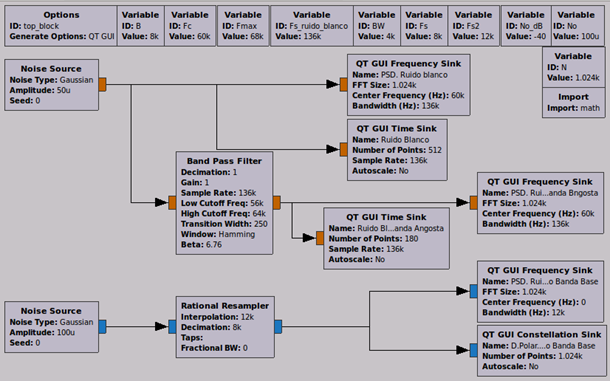
\includegraphics[scale=0.7]{Imagenes/Ruido.png}
	\label{fig:Ruido}
%	\captionsetup{justification=raggedright,font={scriptsize,bf,it}}
%	\caption*{fuente: Tomado del libro de Haykin}
\end{figure}

Los resultados de este flujograma se presentan en la siguiente figura donde podemos ver lo siguiente:

\begin{itemize}
	
	\item [$\bullet$] Hemos puesto un generador de ruido blanco (WN, del inglés White Noise).
	\item [$\bullet$] El ruido blanco en toda su dimensión es imposible de ser observado o simulado, pero podemos obtener una versión con altura de PSD igual a $N_0/2=50 10^{6}$y una frecuencia de muestreo Fs-ruido-blanco=136 KHz, calculando que sea apenas lo suficiente para observar lo que puede ser de interés para nuestro caso. De allí, usando un Filtro Paso Bandas, con ancho de banda B = 8 kHz, hemos obtenido el Ruido Blando de Banda Angosta (NBWN, del inglés Narrow Band White Noise). 
	\item [$\bullet$] Los resultados muestran que, con el filtrado, la señal en el tiempo sufre una caída en la amplitud y su forma se vuelve más suave, pero se conserva la altura de la PSD.\\
	
	\vspace{400px}
	
	\begin{figure}[h!]
		\captionsetup{justification = raggedright, singlelinecheck = false}
		\caption{PDS y señal en el tiempo del ruido blanco (arriba). PSD de la Envolvente compleja ruido blanco de banda angosta y diagrama polar del mismo ruido} 
		\centering
		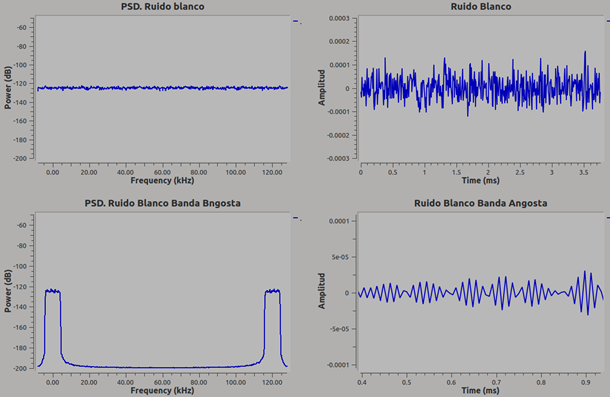
\includegraphics[scale=1]{Imagenes/Ruido-blanco.png}
		\label{fig:Ruido-blanco}
		%	\captionsetup{justification=raggedright,font={scriptsize,bf,it}}
		%	\caption*{fuente: Tomado del libro de Haykin}
	\end{figure}
	
	
	\item [$\bullet$] También hemos usado un generador de ruido blanco en versión compleja con amplitud $N_0=100 10^{6}$, para simular con él lo que debería producir el Down Converter
	\item [$\bullet$] El bloque Rational Resampler se agregó solo con el fin de observar qué hay más allá del ancho de banda bandabase BW=4 kHz. Los resultados, los vemos en la siguiente Figura 45, se trata de la Envolvente Compleja de ruido blanco, que también podemos llamar Ruido Blanco Bandabase. A la izquierda tenemos la PSD y a la derecha la gráfica en el dominio polar.
	
\end{itemize}

%\vspace{250px}
\begin{figure}[h!]
	\captionsetup{justification = raggedright, singlelinecheck = false}
	\caption{Ruido Blanco Banda Base, su PSD y representación Polar} 
	\centering
	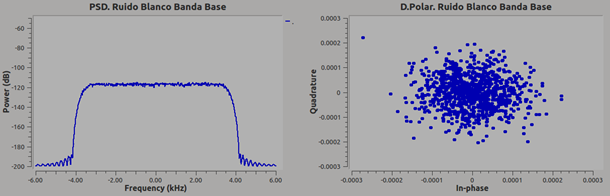
\includegraphics[scale=1]{Imagenes/Polar.png}
	\label{fig:Polar}
	%	\captionsetup{justification=raggedright,font={scriptsize,bf,it}}
	%	\caption*{fuente: Tomado del libro de Haykin}
\end{figure}

\subsection{Un canal inalámbrico de ruido blanco gausiano aditivo en versión bandabase }
El canal de ruido blanco gaussiano aditivo es mejor conocido en inglés como Additive White Gaussian Noise Channel (AWGN Channel). Es bien sabido que una señal en su viaje desde una antena transmisora hasta una receptora atraviesa una gran cantidad de fenómenos. Es como si la señal entrara a un sistema que la deforma de varias maneras y ese sistema es lo que llamamos canal de propagación. Uno de ellos es el ruido y precisamente nos preparamos para revisar cómo luchar contra el efecto que este produce. Es muy claro que si vamos a probar un método para atenuar el ruido blanco, resulta importante poder aislar todos los demás fenómenos que pueden existir en el canal de propagación, de manera que el canal solo tenga la posibilidad de inyectar a la señal ruido blanco. Un esquema práctico es el que se muestra en la figura \ref{fig:Conformacion}.

\begin{figure}[h!]
	\captionsetup{justification = raggedright, singlelinecheck = false}
	\caption{Conformación de un canal pasobandas de ruido blanco.} 
	\centering
	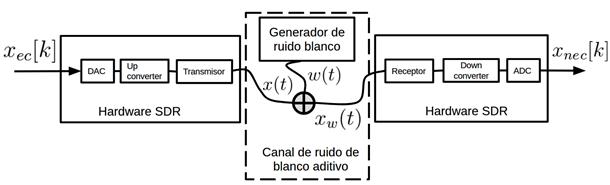
\includegraphics[scale=1]{Imagenes/Conformacion.png}
	\label{fig:Conformacion}
%	\captionsetup{justification=raggedright,font={scriptsize,bf,it}}
%	\caption*{fuente: Tomado de Haykin}
\end{figure}

Como puede verse, el efecto del canal se expresa de la siguiente manera $ x_{w}(t) = x(t) + w(t)$ donde $ x(t) $  es la versión pasobandas y continua de la señal modulada en bandabase , $ x_{ec}[k], w(t) $  es el ruido blanco pasobandas. \\
Cuando se trata de explotar al máximo la posibilidades que ofrece el gnuradio, lo conveniente es crear un canal bandabase de ruido blanco que consiste en imitar prácticamente todos bloques que se tienen en la figura \ref{fig:Conformacion}. Para esto es importante tener en cuenta que la salida de ese canal es $ x_{nec}[k] = x_{ec}[k] + n_{ce}[k] $. \\

Donde $ n_{ce}[k] $ es la envolvente compleja en versión discreta de $n(t)$, el cual a su vez la porción del ruido $ w(t)$ que es admitida por el receptor ya que este tiene un ancho de banda finito y por tanto lo que deja pasar es más bien una señal de ruido blanco de banda angosta , que  llamaremos$  n(t) $. $ n_{ce} [k] $ es conocida también como Ruido Blanco de Banda Angosta en versión Bandabase y discreta. \\

En otras palabras, lo que resulta a la salida del ADC es la misma señal que entra al DAC pero con una adición de ruido blanco banda base , como se muestra en  la figura \ref{fig:Implementacion}, donde se tiene la implementación en GNU Radio de un canal de ruido blanco gaussiano aditivo.\\

\vspace{200px}
\begin{figure}[h!]
\captionsetup{justification = raggedright, singlelinecheck = false}
\caption{Implementación en GNU Radio de un Canal de ruido blanco aditivo.} 
\centering
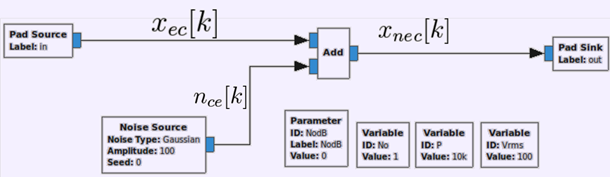
\includegraphics[scale=1]{Imagenes/Implementacion.png}
\label{fig:Implementacion}
%	\captionsetup{justification=raggedright,font={scriptsize,bf,it}}
%	\caption*{fuente: Tomado de Haykin}
\end{figure}

En la figura \ref{fig:Implementacion}, el parámetro Amplitud, en el bloque Noise Source corresponde al valor RMS Vrms del ruido, el cual resulta relacionado con la potencia promedio P del ruido y con el valor No.  \\

En la figura \ref{fig:Diagrama-Polar} se muestra el ruido blanco de banda angosta en banda base, visualizado en un diagrama polar.

\begin{figure}[h!]
	\captionsetup{justification = raggedright, singlelinecheck = false}
	\caption{Ruido Blanco Bandabase en el Diagrama Polar.} 
	\centering
	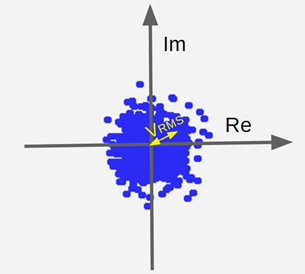
\includegraphics[scale=1]{Imagenes/Diagrama-Polar.png}
	\label{fig:Diagrama-Polar}
	%	\captionsetup{justification=raggedright,font={scriptsize,bf,it}}
	%	\caption*{fuente: Tomado de Haykin}
\end{figure}

Como ya se dijo, el Ruido Blanco es una señal aleatoria teórica, de modo que resulta imposible generarlo en la práctica, pero tampoco resulta necesario generarlo de manera perfecta, pues un receptor, debido a sus limitaciones en ancho de banda solo deja pasar una porción del espectro de ese ruido. En todo caso, al pasar a bandabase, la PSD va a tener una altura constante igual a No, lo cual es fácil de deducir aplicando la Conversión RF vista en el capítulo 1.

\subsubsection{La modulación FM en versión bandabase}
\textcolor{red}{[Falta: Oscar Reyes]} %\OR a nivel de flujograma??
\subsubsection{La modulación AM en versión bandabase}
\textcolor{red}{[Falta: Oscar Reyes]}
%%%%%%%%%%%%%%%%%%%%%%%%%%%%%%%%%%%%%%%
%%%%%%%%%%%%%%%%%%%%%%%%%%%%%%%%%%%%%%%
\section{Ejercicios resueltos}
\subsection{Ejercicio 1}
\subsubsection{Enunciado}
\begin{enumerate}

\item Desde el punto de vista de GNU Radio, ¿de qu\'e tipo es la se\~nal que entrega el USRP receptor atrav\'es de un cable a la computadora?, será:
	\begin{enumerate}
      \item siempre una se\~nal real.
      \item siempre una se\~nal compleja.
      \item por lo general una se\~nal compleja.
	\end{enumerate}
    
\item Teniendo en cuenta que en GNU Radio la siguiente ecuaci\'on puede corresponder a una señal que se entrega a un bloque "UHD: USRP Sink"



\begin{equation} \label{capdos_quince}
S_{ec}[n] = A[n]e^{j(2 \pi  \beta[n]n/(N+Q[n]))}
\end{equation}

Conecte las ecuaciones de envolvente compleja con sus respectivas formas de modulaci\'on mediante una l\'inea recta, cuando en la señal que llega a la antena var\'ia s\'olo:

    \begin{figure} [h!] 
    \centering
    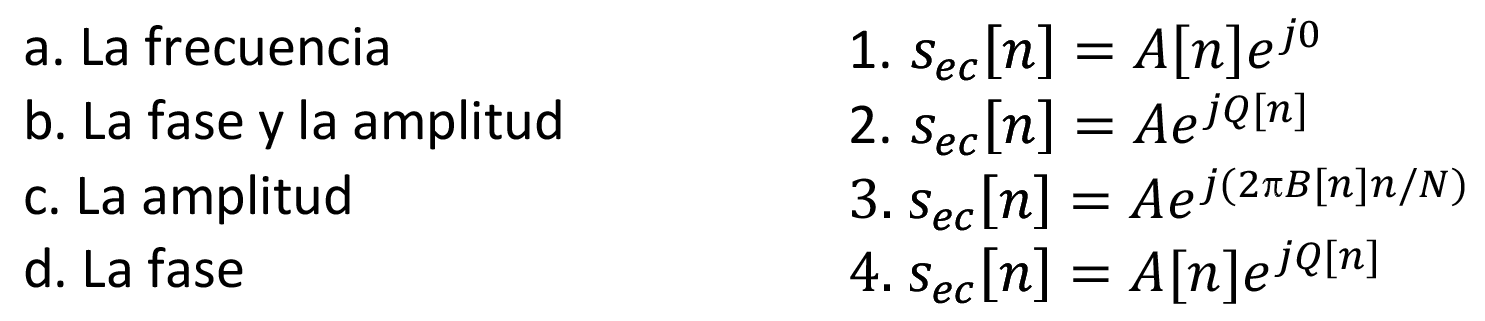
\includegraphics[width=0.7\textwidth]{Imagenes/Comu_1.png}
    \end{figure}

\item Sea la se\~nal $ y(t)=A_{1}\cdot x_{1}(t)\cdot \cos (2\pi ft)+ A_{2}\cdot x_{2}(t)\cdot \sin (2\pi ft+ m(t))$. C\'alcule su envolvente compleja. \\
\end{enumerate}


\subsubsection{Solución}

\begin{enumerate}
\item Rta: (b) Ser\'a siempre una se\~nal compleja.\\
Esto es debido a que el USRP receptor entrega una envolvente, de manera que la señal es inevitablemente compleja en su esencia. Incluso, aún cuando el transmisor emite cero en la parte imaginaria, al receptor llega un cierto ruido en esa parte imaginaria\\
\item Rta:
	\begin{figure} [h!] 
    \centering
    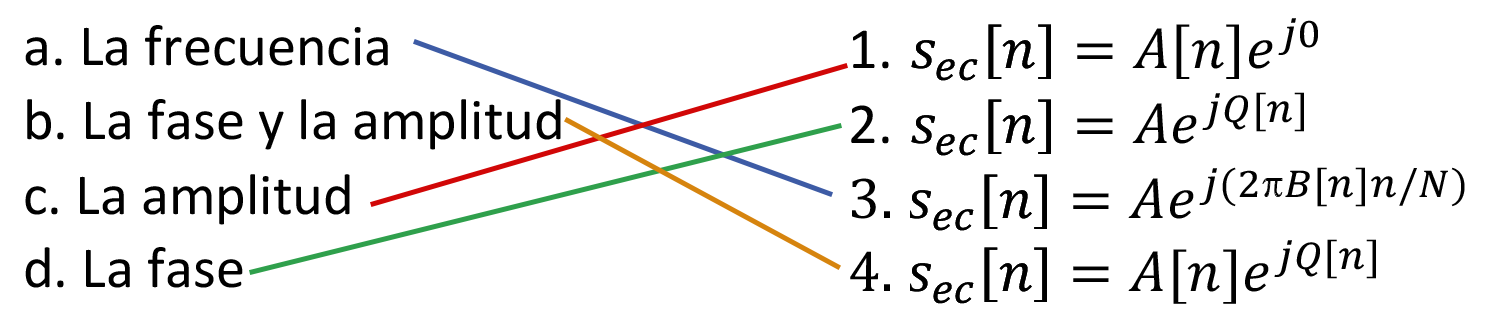
\includegraphics[width=0.7\textwidth]{Imagenes/Comu_1sol.png}
    \end{figure}


%\vspace{1em}
\item Aplicando la definición introducida en este libro de la Conversión RF directa en el dominio del tiempo tenemos:
\\

La definición de la Conversión RF nos indica que:
\begin{equation} \label{capdos_dieciseis}
 A(t)\cdot \cos (2\pi[ f_{0}+B(t)]+Q(t))  \overset{Conversion RF}{\rightarrow} A(t)\cdot e^{j[ \cdot 2\pi B(t)t+Q(t)]}
\end{equation}

Teniendo en cuenta esto, procedemos a calcular la envolvente compleja de la expresión planteada: 

\begin{equation} \label{capdos_diecisiete}
y(t)=A_{1}\cdot x_{1}(t)\cdot \cos (2\pi f_{0}t)+ A_{2}\cdot x_{2}(t)\cdot \sin (2\pi f_{0}t+ m(t))
\end{equation}

Aplicamos Conversión RF a cada termino de la expresión, identificando los parámetros que la conforman. Como lo es la amplitud, frecuencia, fase.\\

Para el término: 
\begin{equation} \label{capdos_dieciocho}
A_{1}\cdot x_{1}(t)\cdot \cos (2\pi ft)
\end{equation}

Encontramos que $A(t) = A_{1} \cdot x_{1}(t),\hspace{1em} f_{c}=f_{0} \hspace{1em} B(t)=0 \hspace{1em} y\hspace{1em} Q(t)=0$\\

Entonces:

\begin{equation} \label{capdos_diecinueve}
 A_{1}\cdot x_{1}(t)\cdot \cos (2\pi ft)  \overset{Conversion \ RF}{\rightarrow} \ 
 A_{1}\cdot x_{1}(t)
\end{equation}

Ahora, para el segundo término: 
\begin{equation} \label{capdos_veinte}
A_{2}\cdot x_{2}(t)\cdot \sin (2\pi f_{0}t+ m(t))
\end{equation}

Encontramos que contiene una función seno, dado que la Conversión RF solo es aplicable a funciones coseno es necesario expresar dicho seno en términos de coseno. Obteniendo el siguiente termino:
\begin{equation} \label{capdos_veintiuno}
A_{2}\cdot x_{2}(t)\cdot \cos (2\pi f_{0}t + m(t)-\pi/2)
\end{equation}

Al identificar los parámetros obtenemos que: \\$A(t) = A_{2} \cdot x_{2}(t),\hspace{1em} f_{c}=f_{0} \hspace{1em} B(t)=0 \hspace{1em} y\hspace{1em} Q(t)=m(t)-\pi/2$\\

Entonces:
\begin{equation} \label{capdos_veintidos}
 A_{2}\cdot x_{2}(t)\cdot \cos (2\pi f_{0}t + m(t) -\pi/2)  \overset{Conversion RF}{\rightarrow} A_{2}\cdot x_{2}(t)\cdot e^{j[ m(t)-\pi/2]}
\end{equation}
Teniendo la envolvente compleja de cada uno de los términos que comprenden y(t), los sumamos para construir su envolvente compleja, obteniendo el siguiente termino como resultado final.

\begin{equation} \label{capdos_veintitres}
 y_{ec}(t)=A_{1}\cdot x_{1}(t) + A_{2}\cdot x_{2}(t)\cdot e^{j[m(t)-\pi/2]}
\end{equation}

\end{enumerate}
%%%%%%%%%%%%%%%%%%%%
\subsection{Ejercicio 2}
\subsubsection{Enunciado}
\begin{itemize}
 \item[1)] Se tiene la siguiente expresión matemática de la envolvente compleja de una señal con modulación digital paso bandas:
 \end{itemize}
 
\begin{equation} \label{capdos_veinticuatro}
yec(t) = \left\lbrace
\begin{array}{ll}
\textup e^{j\pi /4}, m(t)=1  \\
\textup e^{j5\pi /4}, m(t)=0 
\end{array}
\right.
\end{equation}


\begin{itemize}
 \item[a)] Dibujar la EC de la forma polar que se obtendrá con GNU Radio en caso de usar muchísimas muestras por símbolo y graficarla de manera que parezca continua.
 \end{itemize}
 
\begin{itemize}
 \item[b)] Dibujar la EC de la forma polar para el caso en que ella ha sido muestreada, de forma que hay sólo una muestra por bit.
 \end{itemize}


\begin{itemize}
 \item[c)] Dibujar la señal paso bandas que corresponde a la EC dada para los siguientes bits:
 \\
 0 1 1 0
 \end{itemize}

\begin{itemize}
 \item[d)] Dibujar el flujograma gnuradio  para poder transmitir la señal al aire.
 \end{itemize}
 
 \begin{itemize}
 \item[e)] Graficar la forma de la señal en tiempo  que se obtiene en el receptor luego de pasar por el bloque USRP Source.
 \end{itemize}



\subsubsection{Solución}

 \begin{itemize}
 \item[a)]Se puede deducir de la expresión matemática que corresponde a la envolvente compleja de una BPSK, ya que tiene dos fases, una por cada símbolo digital que lleva.


 \begin{equation} \label{capdos_veinticinco}
 X1=45^{\circ}=\frac{\pi }{4} \; ; Para\; los\; unos.
 \end{equation}
 
 \begin{equation} \label{capdos_veintiseis}
 X2= \frac{5\pi }{4}=225^{\circ}; \;	Para\; los\; ceros.
 \end{equation}

%\vspace{100px} 
\begin{figure}[h!]
	\captionsetup{justification = raggedright, singlelinecheck = false}
	\caption{Gráfica de la forma polar continua de la envolvente compleja}
		\centering
    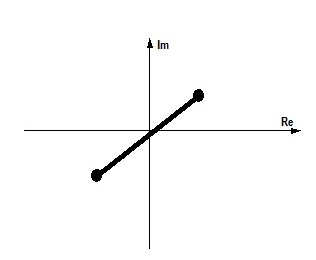
\includegraphics[width=0.8\textwidth]{Imagenes/polarcont.png}
    \label{fig:polarcont}
\end{figure}


\end{itemize}

 \begin{itemize}
 \item[b)] Desde el punto de vista teórico, la señal sólo tiene dos posibles valores, pero en la implementación en GNU Radio, la constelación tiene la forma de una línea debido a la transición cuando la señal pasa de un símbolo a otro.

\vspace{200px} 
 \begin{figure}[h!]
	\captionsetup{justification = raggedright, singlelinecheck = false}
    \caption{Gráfica de la forma polar discreta de la envolvente compleja}
    \centering
    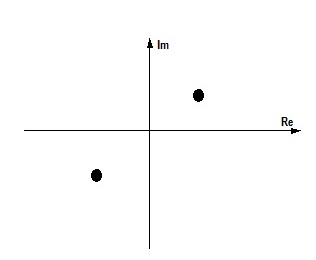
\includegraphics[width=0.8\textwidth]{Imagenes/imagen1.jpg}
    \label{fig:imagen1}
\end{figure}

 \end{itemize}
 
\begin{itemize}
\item[c)] Para la realización de la señal paso bandas es necesario mirar la localización de los cambios de fase de la BPSK en la señal coseno, para saber de esta manera la posición del uno y del cero.

 \begin{figure}[h!]
	\captionsetup{justification = raggedright, singlelinecheck = false}
    \caption{figura de una señal senoidal con su respectiva fase}
    \centering
    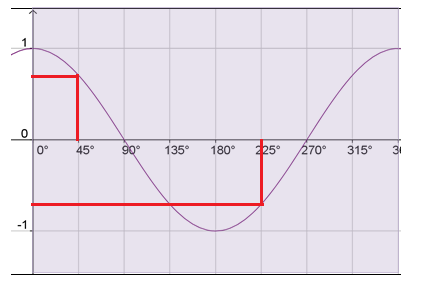
\includegraphics[width=0.8\textwidth]{Imagenes/fas.PNG}
    \label{fig:fas}
\end{figure}

Otra manera de realizar la gráfica de la señal paso bandas es realizar el calculo mediante la Conversión RF. Mediante la cual se puede ver claramente cual es desfase de la señal para cuando tiene u valor de 1 o 0.
\\
\\
La siguiente es la definición de la Conversión RF:
 \begin{equation} \label{capdos_veintisiete}
A(t)cos(2\pi fc*t+B(t)+Q(t))\rightarrow A(t)e^{j(2\pi B(t)+Q(t))}
 \end{equation}
 Aplicando la Conversión RF a $y_{ec}(t)$, tenemos:
\\
Para m(t)=1
 \begin{equation} \label{capdos_veintiocho}
cos(2\pi fc*t+\pi /4)
\end{equation}
\\
Para m(t)=0
 \begin{equation} \label{capdos_veintinueve}
cos(2\pi fc*t+5\pi /4))
\end{equation}
\\

 \begin{figure}[h!]
	\captionsetup{justification = raggedright, singlelinecheck = false}
    \caption{Señal paso banda.}
    \centering
    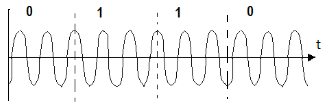
\includegraphics[width=0.8\textwidth]{Imagenes/bit.PNG}
    \label{fig:bit-taller}
\end{figure}


\end{itemize}
 
\begin{itemize}
\item[d)]
 Para la realización de este punto se debe tener en cuenta que lo que se esta transmitiendo son bits que son apenas unos números discretos por consiguiente se necesita un wave forming que en este caso sera un retenedor de orden cero, el cual ayuda a que la señal consiga una forma cuadrada. Ver Figura \ref{fig:ejerciciodiagbloq}. El siguiente bloque corresponde a una constante de multiplicación la cual nos ayuda a atenuar o amplificar la señal según lo requiera el USRP, también se hace uso de un Rational Resampler el cual me permite cuadrar la frecuencia de muestreo a una que sea permitida por el USRP y por ultimo el USRP sink.
 
 \begin{figure}[h!]
	\captionsetup{justification = raggedright, singlelinecheck = false}
    \caption{Diagrama de bloques.}
    \centering
    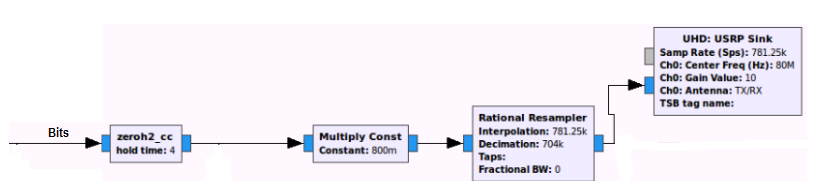
\includegraphics[width=0.8\textwidth]{Imagenes/bloques.png}
    \label{fig:ejerciciodiagbloq}
\end{figure}

\end{itemize}



\begin{itemize}
\item[e)] La Señal en tiempo a la salida del USRP se presenta en la Figura \ref{fig:senalesperadausrp}.Cabe aclarar que la gráfica en GNU Radio no tendrá un aspecto como el de la imagen anterior sino que se observa una gráfica para la parte real, una para la imaginaria y una para la constelación, por aparte. 
\vspace{300px}
 \begin{figure}[h!]
	\captionsetup{justification = raggedright, singlelinecheck = false}
    \caption{Gráfica de la señal en tiempo que se espera a la salida del USRP.}
    \centering
    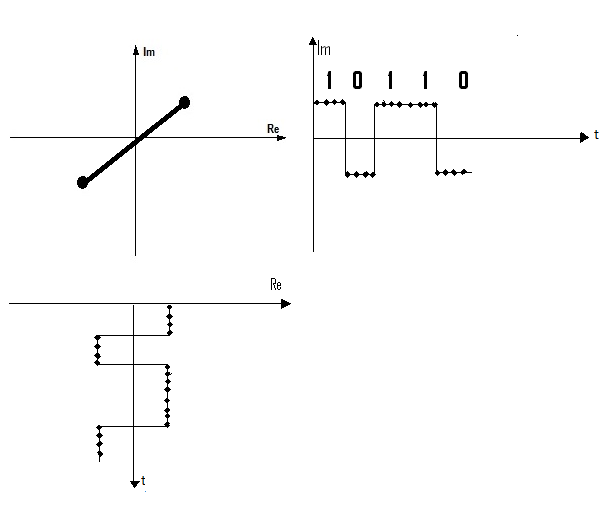
\includegraphics[width=0.8\textwidth]{Imagenes/finalll.png}
    \label{fig:senalesperadausrp}
\end{figure}



\end{itemize}

%%%%%%%%%%%%%%%%%%%%%%%%%%%%%%%%%%%%%%%
\subsection{Ejercicio 3}
\subsubsection{Enunciado}

Se tiene la señal paso banda mostrada en la figura 1. la cual fue obtenida en la entrada de una antena, cuando se deseó transmitir una señal digital. En ella se puede apreciar la forma en que están siendo representados los unos y ceros de la señal y la duración de cada bit.( $T_{b}=0.062ms$). Es importante tener en cuenta que pueden haber mas ciclos por símbolo.\\\\

%\vspace{300px}
 \begin{figure}[h!]
	\captionsetup{justification = raggedright, singlelinecheck = false}
    \caption{Señal pasobanda.}
    \centering
    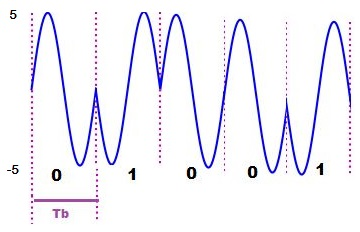
\includegraphics[width=0.5\textwidth]{Imagenes/pasobanda.JPG}
    \label{fig:senaldeceros}
\end{figure}



Teniendo en cuenta lo anterior encuentre la representación polar  de la envolvente compleja de la señal dada.\\

Obtenga la gráfica  de  la PSD (Densidad espectral de potencia) de la señal dada con todas sus  especificaciones, calculando correctamente sus parámetros  para el caso en que la señal de la Figura 1 tiene asignado un canal inalámbrico entre 968 kHz y 1032 kHz.

\subsubsection{Respuesta}

 \begin{figure}[h!]
	\captionsetup{justification = raggedright, singlelinecheck = false}
    \caption{Señal pasobanda que representa a los unos.}
    \centering
    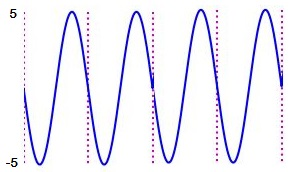
\includegraphics[width=0.6\textwidth]{Imagenes/unos.JPG}
    \label{fig:senaldeunos}
\end{figure}

\begin{equation} \label{capdos_treinta}
c_{1}(t)=5cos(2\pi ft+\frac{\pi}{2})
\end{equation}


 \begin{figure}[h!]
	\captionsetup{justification = raggedright, singlelinecheck = false}
    \caption{Señal pasobanda que representa a los ceros.}
    \centering
    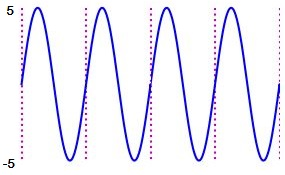
\includegraphics[width=0.6\textwidth]{Imagenes/ceros.JPG}
    \label{fig:respuestadeunos}
\end{figure}

\begin{equation}  \label{capdos_treintauno}
c_{2}(t)=5cos(2\pi ft+\frac{3\pi}{2})
\end{equation}

La transformada Conversión RF directa nos señala que :

\begin{equation} \label{capdos_treintados}
A(t)cos\{2\pi(fc+B(t))t+Q(t)\}\longrightarrow A(t)e^{j(2\pi B(t)t+Q(t))}
\end{equation}
\\

En nuestro caso se tiene que:
\begin{align*}
A(t)=5
\end{align*}
\begin{align*}
B(t)=0
\end{align*}
\begin{align*}
fc=f
\end{align*}

\begin{equation} \label{capdos_treintatres}
Q(t)= \left\{ \begin{array}{lcc}
             \frac{\pi}{2} & = Para\ c_{1}(t) \\
             \\ \frac{3\pi}{2} & = Para\ c_{2}(t) \\
            
             \end{array}
   \right.
\end{equation}\\

Transformada Conversión RF para los unos se tiene:

\begin{equation} \label{capdos_treintacuatro}
c_{1}(t)=5cos(2\pi ft+\frac{\pi}{2})\longrightarrow 5e^{j\frac{\pi}{2}}
\end{equation}

Aplicando la transformada Conversión RF para los ceros se tiene:

\begin{equation} \label{capdos_treintacinco}
c_{2}(t)=5cos(2\pi ft+\frac{3\pi}{2})\longrightarrow 5e^{j\frac{3\pi}{2}}
\end{equation}



Envolvente compleja:

\begin{equation} \label{capdos_treintaseis}
Sec(t)= \left\{ \begin{array}{lcc}
             5e^{j\frac{\pi}{2}}   & = para los unos \\
             \\5e^{j\frac{3\pi}{2}} & = para los ceros \\
            
             \end{array}
   \right.
\end{equation}


 \begin{figure}[h!]
	\captionsetup{justification = raggedright, singlelinecheck = false}
    \caption{Envolvente compleja en un plano polar.}
    \centering
    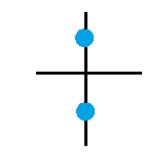
\includegraphics[width=0.4\textwidth]{Imagenes/envolventecompleja.JPG}
    \label{fig:imagendepuntos}
\end{figure}


Calculo de la PSD 
\begin{equation*}
B= 1032kHz - 968kHz = 64 KHz 
\end{equation*} 
\begin{equation*}
Fc=968 kHz + B/2 =968 kHz +32 kHz=1000 kHz
\end{equation*}
\begin{equation*}
Rb=\frac{1}{Tb}=\frac{1}{0.062ms}=16kHz
\end{equation*}
\begin{equation*}
Nlobp=\frac{B}{Rb}=\frac{64kHz}{16KHz}=4
\end{equation*}

\vspace{200px}
 \begin{figure}[h!]
	\captionsetup{justification = raggedright, singlelinecheck = false}
    \caption{Grafica de la PSD.}
    \centering
    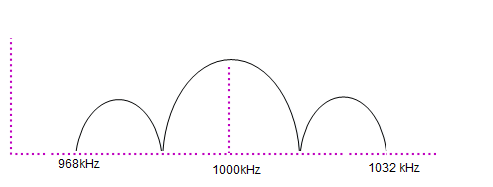
\includegraphics[width=0.8\textwidth]{Imagenes/PSDD.png}
    \label{fig:graficaPSD}
\end{figure}
%%%%%%%%%%%%%%%%%%%%%%%%%%%%%%%%%%%%%%%
\subsection{Ejercicio 4}
\subsubsection{Enunciado}
Se cuenta con un sistema de modulaci\'on pasobandas representado por la interconexi\'on de la figura 1. b(t) es una se\~nal de voltaje continuo que entrega 1V durante un periodo $T_{b}$ para se\~nalar los unos y 0V para se\~nalar los ceros.\\

%\vspace{200px}


 \begin{figure}[h!]
	\captionsetup{justification = raggedright, singlelinecheck = false}
    \caption{Sistema de modulaci\'on pasobandas.}
    \centering
    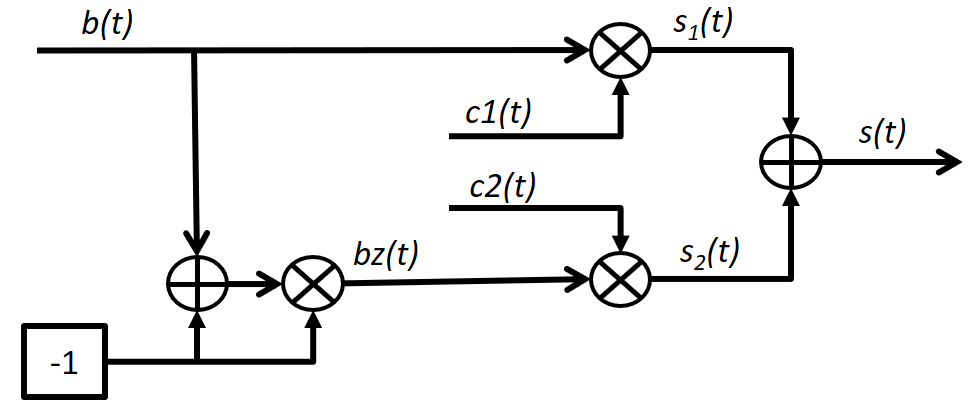
\includegraphics[width=0.6\textwidth]{Imagenes/1.png}
    \label{fig:imagenuno}
\end{figure}

Se tienen los siguientes par\'ametros:\

\[ c_{1}(t)=A_{1}Cos(2\pi f_{1}t) \]
\[ c_{2}(t)=A_{2}Cos[2\pi(f_{1}+\Delta f)t] \]
\[A_{1}=10V \]
\[A_{2}=10V \]
\[f_{1}=1000KHz \]
\[\Delta F=96KHz  \]
\[T_{b}=0,0625ms  \]
$b(t)$ lleva informaci\'on binaria: $ 1,1,0,1,0,0  $
\[B=192KHz \]

Nota: B es un ancho de banda pasobanda.
\begin{itemize}


 \item[a)] Grafique, en funci\'on del tiempo, las se\~nales $s_{1}(t)$,$ s_{2}(t)$ y s(t) para los datos dados. 
 
\item[b)] Grafique la PSD de s(t) se\~nalando todos los par\'ametros con cifras y unidades de medici\'on.
\item[c)] Grafique la envolvente compleja de la se\~nal s(t).
\subsubsection{Respuesta}
 \item[a)]  
Para la soluci\'on del enunciado lo primero que se debe hacer es un bosquejo de la se\~nal mensaje b(t), para ello se tiene en cuenta la informaci\'on binaria que da el enunciado: 1,1,0,1,0,0\
la se\~nal tendr\'ia la siguiente forma:

\vspace{20px}
 \begin{figure}[h!]
	\captionsetup{justification = raggedright, singlelinecheck = false}
    \caption{Mensaje transmitido.}
    \centering
    \includegraphics[width=0.4\textwidth]{Imagenes/2.eps}
    \label{fig:mensajetrans}
\end{figure}

%\newpage
La se\~nal anterior tiene la forma de una codificaci\'on binaria NRZ unipolar en donde al recibir un 1 el flanco sube, mientras que con los ceros ocurre lo contrario. $T_{b}$ es el tiempo del bit.
\
 \item[*]El bosquejo de $s_{1}(t)$  es el resultado de multiplicar la portadora $c_{1}(t)$ por la se\~nal de entrada.

 \begin{figure}[h!]
	\captionsetup{justification = raggedright, singlelinecheck = false}
    \caption{Se\~nal $s_{1}(t)$ en el dominio tiempo }
    \centering
    \includegraphics[width=0.5\textwidth]{Imagenes/3.eps}
    \label{fig:dominiotiempo}
\end{figure}


 \item[*]De igual forma $s_{2}(t)$ es el resultado de multiplicar la portadora $c_{2}(t)$ por la se\~nal $b_{z}(t)$ la cual es la se\~nal resultante de pasar el mensaje por un extractor de ceros como el de la figura 4. \\
 
 \vspace{200px}
 
  \begin{figure}[h!]
	\captionsetup{justification = raggedright, singlelinecheck = false}
    \caption{Extractor de ceros.}
    \centering
    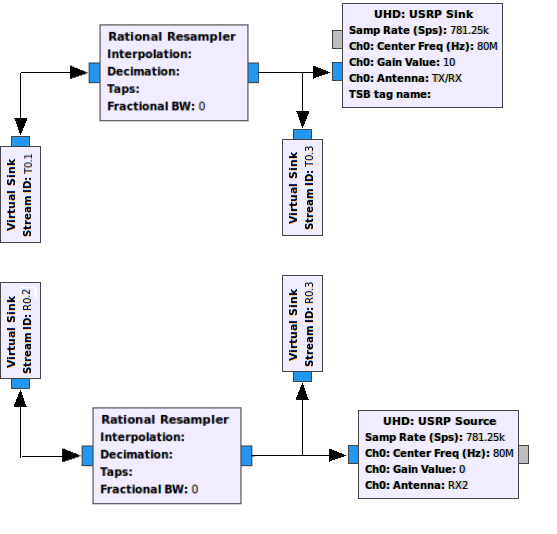
\includegraphics[width=0.6\textwidth]{Imagenes/4.png}
    \label{fig:extractoceros}
\end{figure}
 
El extractor de ceros b\'asicamente lo que hace es convertir los unos a ceros y los ceros a unos. La se\~nal $s_{2}(t)$ la apreciamos en la figura \ref{fig:ejerciciosenals2}.
 
  \begin{figure}[h!]
	\captionsetup{justification = raggedright, singlelinecheck = false}
    \caption{Se\~nal $s_{2}(t)$ en el dominio tiempo }
    \centering
    \includegraphics[width=0.6\textwidth]{Imagenes/6.eps}
    \label{fig:ejerciciosenals2}
\end{figure}

%\newpage
\item[*]Por \'ultimo, se obtiene la se\~nal s(t) que es la suma de $s_{1}(t)$ con $s_{2}(t)$ y se puede apreciar a continuaci\'on:

 \vspace{200px}
   \begin{figure}[h!]
	\captionsetup{justification = raggedright, singlelinecheck = false}
    \caption{Se\~nal s(t) en el dominio tiempo  }
    \centering
    \includegraphics[width=0.6\textwidth]{Imagenes/5.eps}
    \label{fig:ejerciciosenals}
\end{figure}

 
\item[b)]Para graficar la PSD lo primero que se debe hacer es calcular la rata de bits $R_{b}$.\\

\begin{equation} \label{capdos_treintasiete}
 R_{b}=\dfrac{1}{T_{b}}=\dfrac{1}{0.0625*10^{-3}}
\end{equation}

\textbf{Consideraciones para realizar las gráficas de PSD} 
\item[*] Para dibujar la PSD se debe tener en cuenta que el l\'obulo central vale por 2 y est\'a centrado en la frecuencia de portadora.
\item[*] Las PSD de $s_{1}(t)$ y de $s_{2}(t)$ ser\'an iguales pero estar\'an centradas en diferentes frecuencias .   
\item[*] La PSD de una se\~nal pasobandas compuesta por la suma de dos se\~nales de diferentes frecuencias de portadora: $f_{1}$ y $f_{2}$ se obtiene al sumar las PSD de $s_{1}(t)$ y $s_{2}(t)$. \

Teniendo en cuenta lo anterior, se calcula el n\'umero de l\'obulos que tendr\'a la PSD de cada una de las se\~nales $s_{1}(t)$ y $s_{2}(t)$. Se tiene un ancho de banda de 192KHz, el cual se debe repartir entre las dos se\~nales, por lo tanto el ancho de banda que ocupa cada se\~nal es de $ \dfrac{B}{2}.$

\begin{equation} \label{capdos_treintaocho}
 Nlob= \dfrac{ \dfrac{B}{2} }{R_{b}} 
 = \dfrac{ 96[KHz]}{16 [Kbps]} 
 = 6 
\end{equation}

Como se  mencion\'o anteriormente, la PSD de la se\~nal s(t) es el resultado de la suma de las PSD de $s_{1}(t)$ y $s_{2}(t)$; por esto, la PSD de s(t) tendr\'a 12 l\'obulos como se observa a continuaci\'on:

   \begin{figure}[h!]
	\captionsetup{justification = raggedright, singlelinecheck = false}
    \caption{PSD de la se\~nal s(t).}
    \centering
    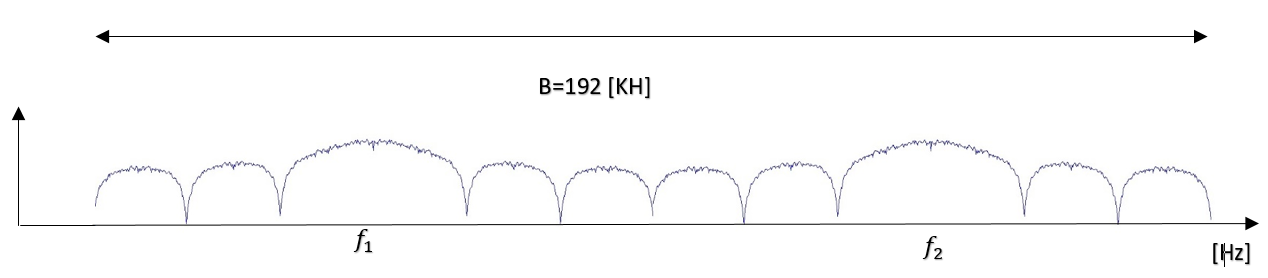
\includegraphics[width=0.7\textwidth]{Imagenes/7.png}
    \label{fig:lobulos}
\end{figure}

Donde:

\[f_{1}=1000KHz \]
\[\Delta f=96KHz  \]
\[f_{2}= f_{1} + \Delta F=  1096 KHz \]

\item[c)] 
\textbf{CONSIDERANDOS}\\
La diferencia entre una se\~nal bandabase (envolvente compleja) y la correspondiente pasobandas se puede observar en las figuras 8 y 9.

 \begin{figure}[h!]
	\captionsetup{justification = raggedright, singlelinecheck = false}
    \caption{PSD banda base.}
    \centering
    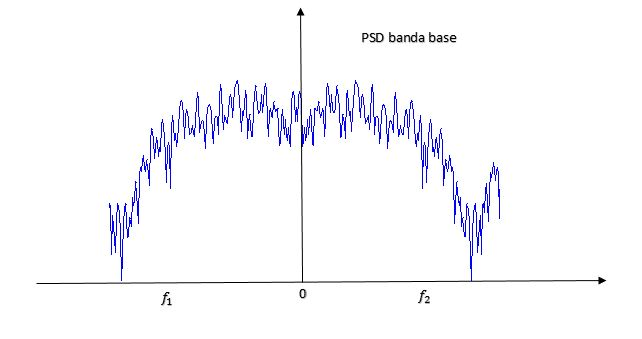
\includegraphics[width=0.6\textwidth]{Imagenes/9.jpeg}
    \label{fig:lobuloconsi}
\end{figure}


 \begin{figure}[h!]
	\captionsetup{justification = raggedright, singlelinecheck = false}
    \caption{PSD pasobandas.}
    \centering
    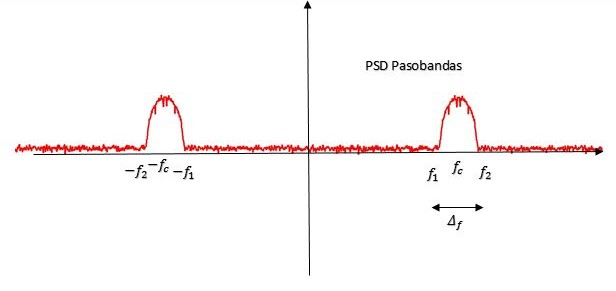
\includegraphics[width=0.6\textwidth]{Imagenes/10.jpeg}
    \label{fig:lobulodos}
\end{figure}

%\newpage
Para encontrar la envolvente compleja a partir de la se\~nal s(t) se usa la transformada RF (Conversión RF) que se define de la siguiente manera:\

\begin{equation}  \label{capdos_treintanueve}
A(t) Cos[ 2\pi(fc + B(t)) t + Q(t)] \\\\
\dfrac{Conversion RF}{} > A(t) e^{j[ 2\pi B(t) t + Q(t)]}  
\end{equation}

Aplicando la transformada Conversión RF se tiene:

\begin{equation}  \label{capdos_cuarenta}
s(t) = c_{1}(t) +c_{2}(t)
\end{equation}

\begin{equation}  \label{capdos_cuarentayuno}
 c_{1}(t)= A_{1} Cos [2\pi  (fc-\dfrac{\Delta F}{2})]\: para \: b(t)=1 
\end{equation}

\begin{equation}  \label{capdos_cuarentaydos}
 c_{2}(t)= A_{2} Cos [2\pi (fc+\dfrac{\Delta F}{2})] \: para \: b(t)=0 
\end{equation}


En ambos casos $Q(t)=0.$ La expresi\'on de envolvente compleja viene dada por:


\begin{equation}  \label{capdos_cuarentaytres}
c_{1}ce(t)=  A_{1} e^{-j2\pi \dfrac{\Delta F}{2}} \end{equation}

\begin{equation}  \label{capdos_cuarentaycuatro}
c_{2}ce(t)=  A_{2} e^{j2\pi \dfrac{\Delta F}{2}}
\end{equation}

 
 
\item[*] En banda base, la se\~nal es un vector rotante a una velocidad $\hat{f_{1}}$ para los unos y  $\hat{f_{2}}$ para los ceros.\\

%\vspace{20px}
 
\begin{figure}[h!]
	\captionsetup{justification = raggedright, singlelinecheck = false}
    \caption{Envolvente compleja s(t) forma polar.}
    \centering
    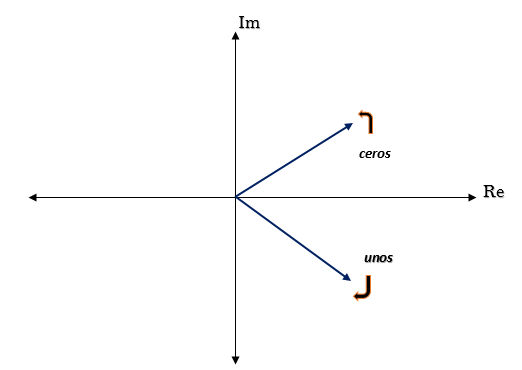
\includegraphics[width=0.6\textwidth]{Imagenes/12.jpeg}
    \label{fig:Envol-polar}
\end{figure}


Como se mencion\'o anteriormente, la envolvente compleja tiene forma de exponencial compleja la cual se puede expresar de la siguiente manera:

\begin{equation}  \label{capdos_cuarentaycinco}
e^{jx} = cos x +j sen x 
\end{equation}

Por lo tanto, para dibujar la parte real de la envolvente compleja se parte de la se\~nal coseno de la \textcolor{Red}{figura 11}  y para dibujar la parte imaginaria de la envolvente compleja se parte de la se\~nal seno de la \textcolor{Red}{figura 12.} 
 
\begin{figure}[h!]
	\captionsetup{justification = raggedright, singlelinecheck = false}
    \caption{Se\~nal a partir de la cual se dibuja la parte real de la envolvente compleja.}
    \centering
    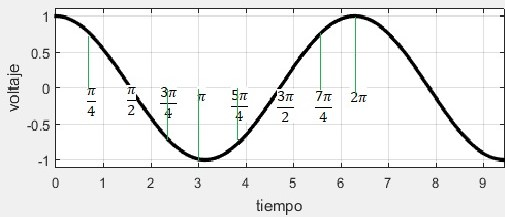
\includegraphics[width=0.8\textwidth]{Imagenes/15.jpeg}
    \label{fig:seno-ejercicio}
\end{figure}

\vspace{200px}
\begin{figure}[h!]
	\captionsetup{justification = raggedright, singlelinecheck = false}
    \caption{Se\~nal a partir de la cual se dibuja la parte imaginaria de la envolvente compleja.}
    \centering
    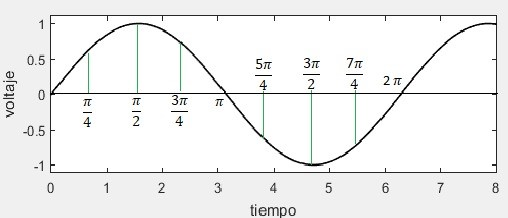
\includegraphics[width=1\textwidth]{Imagenes/16.jpeg}
    \label{fig:matlab-ejercicio}
\end{figure}

%\newpage 

Finalmente, se tiene que la envolvente compleja de la se\~nal s(t) es: 

\begin{figure}[h!]
	\captionsetup{justification = raggedright, singlelinecheck = false}
    \caption{Envolvente compleja s(t).}
    \centering
    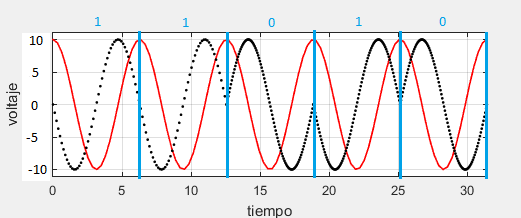
\includegraphics[width=1\textwidth]{Imagenes/13.png}
    \label{fig:dos-senos}
\end{figure}

 
En la figura anterior, para no dibujar demasiados ciclos en $T_{b}$, la gr\'afica a sido simplificada a un ciclo en $T_{b}$, sin embargo en la pr\'actica hay $ \dfrac{\Delta F}{2} $ ciclos en $T_{b}$.
\end{itemize}